%!TEX root = thesis.tex
\chapter{Fundamentals of nematic liquid crystals}\label{c:2}

\section{Local order and defects}
Uniaxial nematic liquid crystals are an ordered phase resulting from breaking the continuous rotational symmetry of a collection of anisotropic, typically rod-like or plate-like, particles~\cite{RN33}.
As either the concentration of the particles is increased~\cite{RN204} or the temperature of the system is decreased~\cite{RN202}, there is a point where a phase transition happens and the system breaks continuous rotational symmetry and develops order.
The order is characterized by a spontaneously chosen preferred direction or axis; rod-like particles prefer to have their long axis aligned along this direction and plate-like particles prefer to have their short axis along this direction~\cite{RN33,RN175}.

Note that the system still possesses continuous rotational symmetry about the preferred alignment direction as well as continuous translational symmetry in  all directions.
This is illustrated with rod-like particles in Figure~\ref{f:2-NematicSym}.
In panel (A), the system is isotropic and there is no preferred alignment direction.
In contrast, in panels (B) and (C), the rods now align along a preferred direction denoted by $\mathbf{n}$ and called the director.
As a result, in Figure~\ref{f:2-NematicSym}(B) and Figure~\ref{f:2-NematicSym}(C), the system has broken continuous rotational symmetry about the two axes orthogonal to $\mathbf{n}$.
Note that even though in Figure~\ref{f:2-NematicSym}(C) the rods align more strongly along $\mathbf{n}$ than the rods in Figure~\ref{f:2-NematicSym}(B), the system possesses the same symmetry in both situations.

Regardless of the rotational symmetry of the system, the system never breaks translational symmetry.
This can be seen in Figure~\ref{f:2-NematicSym}(D), where we show the centers of mass of the rods for all the cases in Figure~\ref{f:2-NematicSym}(A--C), illustrating that there is no positional order and the system still possesses continuous translational symmetry.
If the concentration of the particles were further increased or the temperature were further decreased, the system would eventually break translational symmetry and the nematic phase would transition to a crystalline phase, with three broken continuous translational symmetries~\cite{RN33}.
Hence, the liquid-crystalline nematic phase is an intermediate ``mesophase'' that possesses the continuous translational symmetries of the isotropic ``liquid phase'' as well as some of the broken rotational symmetries of the ``crystalline'' phase.

We briefly mention that nematics can be biaxial instead of uniaxial.
Here, the constituent particles are bar-like such that there is no longer a single axis of symmetry that can characterize the particle geometry~\cite{RN33,RN175}.
Instead, we would need to define two axes, hence the name biaxial.
However, in this Thesis, we will focus only on uniaxial NLC whose constituent particles are rod-like.

\begin{figure}[h]
  \centering
  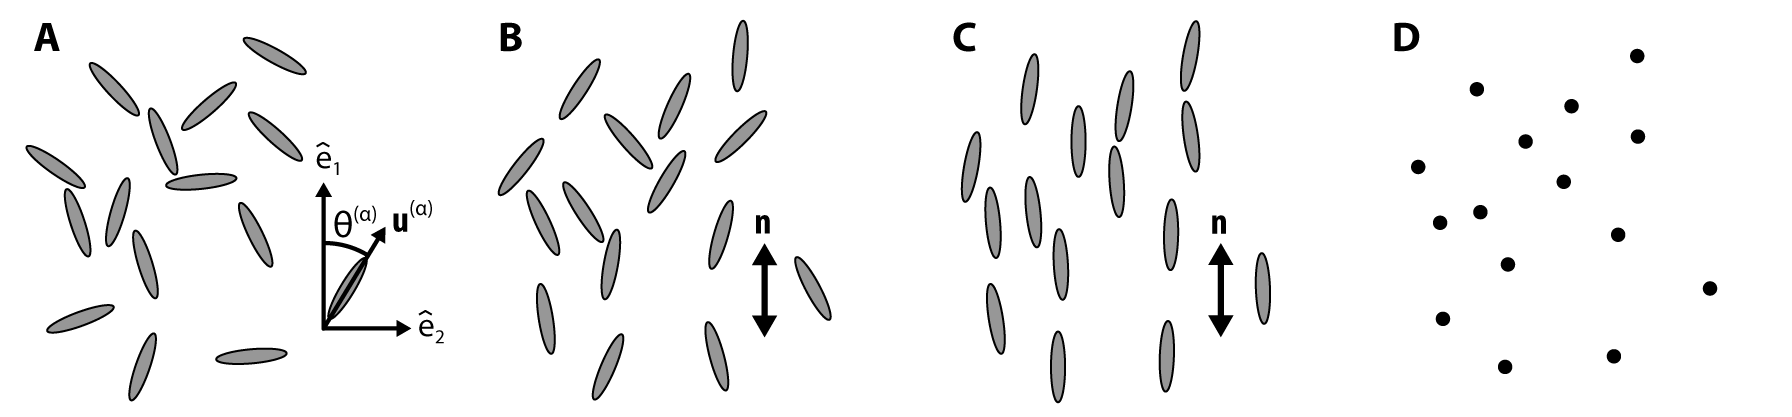
\includegraphics{figures/C2/Ch2-Figs_NematicSym.png}
  \caption{ Symmetries in nematic phase. (A), A collection of rod-like particles in the isotropic phase.
  The orientation of the rod with index $\alpha$ is given by the angle $\mathbf{u}^{\alpha}$, defined schematically in the image.
  (B), The rods from (A) in the nematic phase.
  The rods are preferentially but weakly aligned along the director $\mathbf{n}$, denoted in the panel.
  (C), The rods from (A,B) in the nematic phase. Here, the rods are strongly aligned along $\mathbf{n}$, denoted in the panel.
  (D), The positions of the center of mass of the rods in (A--C), highlighting the continuous translational symmetry of the rods.}\label{f:2-NematicSym}
\end{figure}

\subsection{The director and the order parameter}
Given a group of rods, we want to determine if the system is in the isotropic or the nematic phase, in addition to finding the director, $\mathbf{n}$, provided that the rods are in the nematic phase.
Since we have a collection of rods with no specified head nor tail, the director has inversion symmetry such that $\mathbf{n} = -\mathbf{n}$ and $\mathbf{n}\cdot\mathbf{n} = 1$.
Thus, to indicate nematic order, we need an order parameter that goes to $0$ in the isotropic phase, is nonzero in the nematic phase, and describes the broken symmetry~\cite{RN33,RN175}.
We will first derive this quantity for a collection of rods laying in a 2D plane and then generalize to rods in 3D.
Let a 2D collection of rods laying in a plane be indexed by $\alpha = 1,2,\dots, N$, such that the orientation of a given rod can be specified with the unit vector $\mathbf{u}^{(\alpha)} = u^{(\alpha)}_i\hat{e}_i$, as seen in Figure~\ref{f:2-NematicSym}(A), where we use the Einstein summation convention to sum over repeated indices and $\{\hat{e}_1,\hat{e}_2  \}$ is the standard basis in $\mathbb{R}^2$.
Note that due to the inversion symmetry of the nematic phase $\langle \mathbf{u}^{(\alpha)}\rangle_{\alpha} = 0$, where $\langle \cdot \rangle_{\alpha}$ represents an ensemble average over all $\alpha$.
Thus, to accommodate the $\mathbf{u}^{(\alpha)} = -\mathbf{u}^{(\alpha)}$ inversion symmetry of a nematic, we will construct a symmetric rank-2 tensor from $\mathbf{u}^{(\alpha)}$.
Let:
\begin{equation}
  \mathbf{Q} = \left \langle \mathbf{u}^{(\alpha)} \otimes \mathbf{u}^{(\alpha)} - \frac{1}{2} \mathbb{1} \right \rangle_{\alpha},\label{e:2-2DOrderRaw}
\end{equation}
with $\otimes$ the outer product.
Now, $\textrm{tr}\big \{ \mathbf{Q} \big \} = \langle \mathbf{u}^{(\alpha)} \cdot \mathbf{u}^{(\alpha)} - 1 \rangle_{\alpha} = 0$, making $\mathbf{Q}$ traceless~\cite{RN33,RN175}.
We need $\mathbf{Q}$ to be traceless if we wish to use $\mathbf{Q}$ as an order parameter with $Q_{ij} = 0$ in the isotropic phase.

To determine the director, we need to diagonalize $\mathbf{Q}$.
Without loss of generality, we choose a new orthonormal basis in the plane, $\{ \hat{e}_1', \hat{e}_2' \}$.
The transformation from the unprimed to the primed basis is given by the matrix $V_{ij} = \hat{e}'_i \cdot \hat{e}_j$.
Note that $\mathbf{V}^T \mathbf{V} = V_{ij}V_{jk} =  \mathbb{1}$, implying that $\mathbf{V}^T = \mathbf{V}^{-1}$, and $\mathbf{V}$ is orthogonal.
We then have:
\begin{align}
  \mathbf{Q}' = \mathbf{V} \mathbf{Q} \mathbf{V}^T &=
  \bigg \langle \big ( \mathbf{V} \mathbf{u}^{(\alpha)} \big ) \otimes \big ( \mathbf{V} \mathbf{u}^{(\alpha)} \big )\bigg \rangle_{\alpha}  - \frac{1}{2} \mathbb{1} \nonumber \\ & =
  \begin{pmatrix}
    \langle \cos^2 \theta'^{(\alpha)}\rangle_{\alpha} - 1/2 & \langle \sin \theta'^{(\alpha)} \cos \theta'^{(\alpha)} \rangle_{\alpha} \\
    \langle \sin \theta'^{(\alpha)} \cos \theta'^{(\alpha)} \rangle_{\alpha} & \langle \sin^2 \theta'^{(\alpha)} \rangle_{\alpha} - 1/2
  \end{pmatrix},\label{e:2-2DOrderRot}
\end{align}
where $\cos \theta'^{(\alpha)} = \mathbf{u}^{(\alpha)} \cdot \hat{e}_1'$ and $\sin \theta'^{(\alpha)} = \mathbf{u}^{(\alpha)} \cdot \hat{e}_2'$.

Since $\mathbf{Q}$ is symmetric, we can find a basis of eigenvectors where $\mathbf{Q}'$ is diagonal.
Choose the $\hat{e}'_i$ to be the eigenvectors of $\mathbf{Q}$.
This implies $ \mathbf{V} \mathbf{Q} \mathbf{V}^T$ must be diagonal such that $\langle \sin \theta'^{(\alpha)} \cos \theta'^{(\alpha)} \rangle_{\alpha} = \langle \sin (2 \theta'^{(\alpha)}) \rangle_{\alpha} = 0$.
This can occur in two instances.
First, if we choose the collection of rods to be randomly oriented as in the isotropic phase, $\langle \sin (2 \theta'^{(\alpha)}) \rangle_{\alpha} = 0$ as sine is an odd function.
However, in this case we also have $\langle \cos^2 \theta'^{(\alpha)}\rangle_{\alpha} - 1/2 = \langle \sin^2 \theta'^{(\alpha)}\rangle_{\alpha} - 1/2 = 0$, and thus $\mathbf{Q} = 0$.
This first situation simply shows the correct behavior in the isotropic phase.
The second situation is the one we are seeking.
For $\langle \sin (2 \theta'^{(\alpha)}) \rangle_{\alpha}$ to be $0$, the collection of rods must on average point along $\hat{e}'_i$, implying that $\theta'^{(\alpha)} \approx 0 \textrm{ or } \pi/2$.
This further indicates that $\mathbf{n}$ is either along $\hat{e}_1'$ or along $\hat{e}_2'$, the eigenvectors of $\mathbf{Q}$.

We now take Eq.~\ref{e:2-2DOrderRot} and write it assuming the collection of rods on average points along $\hat{e}'_1$, hence $\mathbf{n} = \hat{e}_1'$.
This yields:
\begin{equation}
  \mathbf{V} \mathbf{Q} \mathbf{V}^T =
  \begin{pmatrix}
    \langle \cos^2 \theta'^{(\alpha)}\rangle_{\alpha} - 1/2 & 0 \\
    0 & \langle \sin^2 \theta'^{(\alpha)} \rangle_{\alpha} - 1/2
  \end{pmatrix} =
  \begin{pmatrix}
    S/2 & 0 \\
    0 & -S/2
  \end{pmatrix},\label{e:2-2DOrderDiagBig}
\end{equation}
where $S = 2 \langle \cos^2 \theta'^{(\alpha)} \rangle_{\alpha} - 1$.
From Eq.~\ref{e:2-2DOrderDiagBig}, we find that the eigenvalue associated to the eigenvector $\hat{e}_1'$ is $S/2$, while for the eigenvector $\hat{e}_2'$ the eigenvalue is $-S/2$.
Since we specified that the rods prefer to align along $\hat{e}_1'$, we see that $\mathbf{n}$ is the eigenvector that corresponds to the largest eigenvalue of $\mathbf{Q}$.
S is often called the scalar order parameter and denotes how well-aligned the system is~\cite{RN33}.
For example, if every rod was aligned along $\hat{e}_1'$ such that $\mathbf{u}^{(\alpha)} = \hat{e}'_1$, $S = 1$.
Similarly, if we again check the isotropic limit of a random collection of rods, we see that $S = 0$, as desired.
Returning to Figure~\ref{f:2-NematicSym}, we see that $S=0$ in Figure~\ref{f:2-NematicSym}(A), and that $0 < S\big[$Figure~\ref{f:2-NematicSym}(B)$\big] < S\big[$Figure~\ref{f:2-NematicSym}(C)$\big] < 1$.
Thus, $\mathbf{Q}$ serves as the tensor order parameter for a collection of rods, where the director corresponds to the eigenvector associated with the largest eigenvalue of $\mathbf{Q}$, and that eigenvalue gives $S$, the scalar order parameter~\cite{RN33,RN175}.

In terms of the director, we can now write $\mathbf{Q}$ in 2D as:
\begin{equation}
  \mathbf{Q} = S \left ( \mathbf{n} \otimes \mathbf{n} - \frac{1}{2}\mathbb{1} \right ).\label{e:2-2DOrderDiag}
\end{equation}
Generalizing to 3D, we have a similar expression for a collection of rods~\cite{RN33}:
\begin{equation}
  \mathbf{Q} =  \left \langle \mathbf{u}^{(\alpha)} \otimes \mathbf{u}^{(\alpha)} - \frac{1}{3} \mathbb{1} \right \rangle_{\alpha},\label{e:2-3DOrderRaw}
\end{equation}
that can be written in terms of the director as:
\begin{equation}
  \mathbf{Q} = S \left ( \mathbf{n} \otimes \mathbf{n} - \frac{1}{3}\mathbb{1} \right ),\label{e:2-3DOrderDiag}
\end{equation}
with $S = \frac{1}{2} \big \langle 3 \cos^2 \theta'^{(\alpha)}  - 1 \big  \rangle_{\alpha} = \big \langle P_2(\cos \theta'^{(\alpha)}) \big \rangle_{\alpha} $,
where again $\theta'^{\alpha} = \arccos (\mathbf{u}^{\alpha} \cdot \mathbf{n})$, and $P_2(\cdot)$ is the Legendre Polynomial of order 2~\cite{RN33,RN175}.
As in two dimensions, we take the eigenvector associated with the largest eigenvalue to be $\mathbf{n}$.
Thus, for a collection of rods, we can determine the phase and, if applicable, $\mathbf{n}$ by calculating $\mathbf{Q}$ according to Eqs.~\ref{e:2-2DOrderRaw} or~\ref{e:2-3DOrderRaw} and diagonalizing.


\subsection{Defects in a nematic}\label{c:2-defects}
While we briefly mentioned the dimensionality of defects and their associated classification schemes in Section~\ref{c:1}, here we take a deeper look and use homotopy theory as laid out in references~\cite{RN196,RN236,RN153} to introduce a more complete theory of defects in nematic materials.
As mentioned in Chapter~\ref{c:1}, defects in ordered media are defined generally as regions where the characteristic order of the phase is not satisfied.
In a nematic phase, defects are locations where $\mathbf{n}$ is undefined.
For a nematic in 3D, these locations can be $0$-dimensional ($0$D) (point defects), $1$-dimensional ($1$D) (line defects), or $2$D (wall defects).
General examples of defects with different dimensionality in 3D and 2D are drawn schematically in Figure~\ref{f:2-GenDef}.
Note that when a 3D defects structure depends only on 2 coordinates, as seen in the invariance along $\hat{z}$ in the wall and line defects in Figure~\ref{f:2-GenDef}, the director in the $xy$ plane appears as if we were in 2D.
For example, a wall in 3D is similar to a line in 2D and a line in 3D is similar to a point in 2D, as highlighted by the arrows in Figure~\ref{f:2-GenDef}.

However, while it is appealing to equate similar-looking structures in 2D and 3D, the additional possible director orientations in a 3D nematic mean that a 3D nematic is fundamentally different than a 2D nematic.
To characterize these differences as well as classify the defects themselves we turn to the homotopy theory of defects.
For clarity, we refer to Table~\ref{t:2-GroupTheory} for definitions of some useful concepts from group theory.\\
\begin{figure}[h]
  \centering
  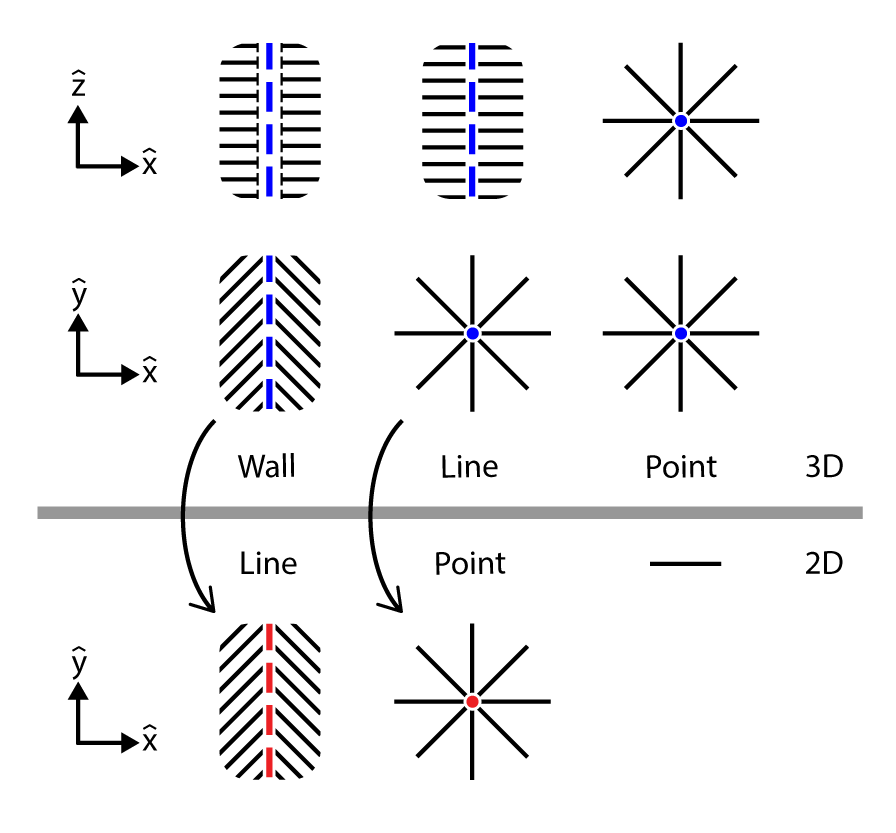
\includegraphics{figures/C2/Ch2-Figs_GenDef.png}
  \caption{Different types of defects in 3D and 2D.
  In 3D, there is the 2D wall defect, the 1D line defect, and the 0D point defect.
  Cross-sections of these three structures are shown schematically in the $xy$ plane and the $xz$ plane.
  The defects are marked with either a dot or a dashed line.
  The head of the``nails'' in the $xz$ cross-section of the wall point into the page.
  In 2D, a nematic can have 1D line defefcts and 0D point defects, where the singular region is highlighted with either a dashed line or a point.
  Note that the wall and line structures in 3D are invariant along the $\hat{z}$-direction.
  This invariance means that the $xy$ cross-section of the wall and line structure in 3D map to the line and point structure in 2D, as shown by the arrows in the schematic.}\label{f:2-GenDef}
\end{figure}

Consider a 2D set of vectors such that their orientations can be described by a single angle.
We can map these vector orientations onto an \emph{order parameter space} given by the 1-sphere, $\mathbb{S}^1$, the unit circle in the plane, such that $\mathbb{S}^1$ describes all the possible orientations of the vectors.
If instead we consider a nematic where $\mathbf{n} = -\mathbf{n}$, $\mathbb{S}^1$ is no longer an appropriate order parameter space as the orientations of $\mathbf{n}$ are periodic on the interval $[0,\pi)$ and not on the interval $[0,2 \pi)$.
Instead, for 2D nematics the order parameter space is $\mathbb{R}\mathbb{P}^1$, the real projective plane in 1D, which corresponds to $\mathbb{S}^1$ with antipodal points identified~\cite{RN196,RN153,RN236}.
This means that specifying the director along a contour in real space will determine a mapping to the order parameter space.

For example, consider both the purple contour and the red contour in the real space director schematic in Figure~\ref{f:2-2DMeas}(A) and their associated mappings to $\mathbb{R}\mathbb{P}^1$ in the schematic in Figure~\ref{f:2-2DMeas}(B,C).
Both contours are closed.
However, we see in Figure~\ref{f:2-2DMeas}(A) that the red contour encloses a singularity while the purple contour does not.
Similarly, we see that in the order parameter space in Figure~\ref{f:2-2DMeas}(B), the purple contour does not span $\mathbb{RP}^1$ and thus can be continuously deformed to a point in $\mathbb{R}\mathbb{P}^1$.
In contrast, the red contour in Figure~\ref{f:2-2DMeas}(C) spans $\mathbb{RP}^1$ and cannot be shrunken continuously to a point.
Thus, the presence of a singularity in the area bounded by the red contour in real space results in a nonzero winding number in the associated contour in the order parameter space.

In fact, it is easy to see that a mapping of the director along the blue contour in Figure~\ref{f:2-2DMeas}(D) will result in a contour in $\mathbb{R}\mathbb{P}^1$ that spans $\mathbb{RP}^1$ and goes in opposite direction to the red contour in  Figure~\ref{f:2-2DMeas}(C).
A mapping of the director to $\mathbb{R}\mathbb{P}^1$ along the green contour in Figure~\ref{f:2-2DMeas}(E) will result in a contour that wraps $\mathbb{R}\mathbb{P}^1$ twice in the same direction as the red contour.
Explicitly, we see that the defect structures in Figure~\ref{f:2-2DMeas}(A,D,E) all have different winding numbers in $\mathbb{R}\mathbb{P}^1$, and thus cannot be mapped onto each other with continuous deformations.
In the language of homotopy theory, we say that any two contours that can be continuously deformed into each other (i.e., via a homeomorphism) are homotopic~\cite{RN196}.
More generally, any contour in $\mathbb{R}\mathbb{P}^1$ with winding number $k$ is homotopic to any other contour in $\mathbb{R}\mathbb{P}^1$ with winding number $k$, and only to contours with winding number $k$~\cite{RN196,RN153,RN236}.
For example, note that as a single point in $\mathbb{R}\mathbb{P}^1$ corresponds to a homogeneous $\mathbf{n}$-field in real space, we see that the singularity-free director field with $k=0$ bounded by the purple contour in Figure~\ref{f:2-2DMeas}(A) is homotopic to the homogeneous state of any orientation, but is not homotopic to the director field with $k=1$ bounded by the red contour in Figure~\ref{f:2-2DMeas}(A).
Thus, contours with the same winding number form a homotopy class, where we can now start to think about categorizing the different homotopy classes of defects using a group structure.

While we could form the group using the winding numbers in $\mathbb{R}\mathbb{P}^1$ themselves, it is more common to use the winding number about $\mathbb{S}^1$ such that the winding number is equivalent to measuring the amount of director rotation around a contour in real space~\cite{RN23,RN153,RN203}.
Reproducing Eq.~\ref{eq:1-topCharge} from Chapter~\ref{c:1} for a director field parametrized by the angle $\phi(\mathbf{r})$, we characterize the defects with their winding number, $s$~\cite{RN153,RN236}:
\begin{equation}
  s = \frac{1}{2 \pi}\oint_{\partial A} \textrm{d}\mathbf{r} \cdot \nabla\phi(\mathbf{r}),\label{eq:2-topCharge}
\end{equation}
where $\partial A$ is the boundary of some area $A$ containing the defect and the integral is performed along the boundary keeping A to the left.
Since we have already established that the defects in a 2D nematic have integer winding numbers in $\mathbb{R}\mathbb{P}^1$, we see that $s = n/2$, with $n \in \mathbb{Z}$, giving us a discrete set of elements.
In addition, we know that winding numbers are additive~\cite{RN196}, such that combining the effect of multiple defects is commutative and associative.
The additivity can be seen in Figure~\ref{f:2-2DMeas}(F), where a contour surrounding two $s = +1/2$ defects has the same winding number in $\mathbb{R}\mathbb{P}^1$ as the contour encircling the single $s = +1$ defect in Figure~\ref{f:2-2DMeas}(E).
Similarly, the additivity of defects also means that the (additive) inverse of a defect with winding number $+k$ is a defect with winding number $-k$.
For example, combining an $s = +1/2$ defect and an $s = -1/2$ defect will result in the homogeneous state.
Finally, we note that the homogeneous state acts as the identity element for the set of defects as $k + 0 = k$.
Since we have satisfied the axioms for a group laid out in Table~\ref{t:2-GroupTheory}, we see that these defects belong to the group $(\mathbb{Z}/2, +)$, the Abelian group formed from the set of half-integers with addition.
Thus, we can characterize the homotopy classes of point defects in $\mathbb{R}\mathbb{P}^1$ with $\pi_1 (\mathbb{R}\mathbb{P}^1) = \mathbb{Z}/2$, the first \emph{homotopy group}, also known as the \emph{fundamental group}, of $\mathbb{R}\mathbb{P}^1$~\cite{RN196,RN153,RN236}.
Hence, the quantity $s$ is a topological quantity often referred to as ``topological charge.''
\begin{figure}[h]
  \centering
  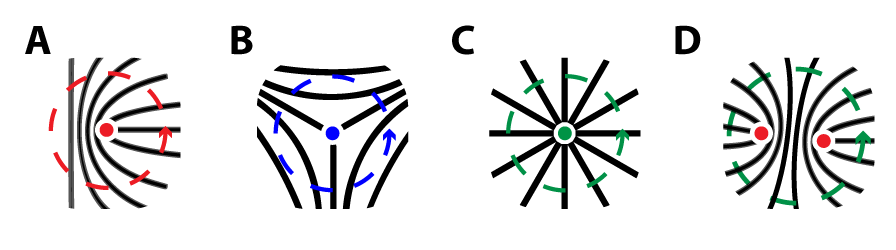
\includegraphics{figures/C2/Ch2-Figs_2DMeas.png}
  \caption{Examples of defect structures and the order parameter space in 2D.
  (A), An $s=+1/2$ defect with the singularity denoted with a red dot.
  The director along the red and purple contours is mapped to $\mathbb{R}\mathbb{P}^1$ in (B).
  (B), A schematic showing $\mathbb{R}\mathbb{P}^1$ (black line) as $\mathbb{S}^1$ (full circle) with antipodal points identified.
  The purple contour in $\mathbb{R}\mathbb{P}^1$ corresponds to the purple contour in real space drawn schematically in (A).
  The purple contour can be continuously deformed to a point in $\mathbb{R}\mathbb{P}^1$.
  (C), A schematic showing $\mathbb{R}\mathbb{P}^1$ (black line) as $\mathbb{S}^1$ (full circle) with antipodal points identified.
  The red contour in $\mathbb{R}\mathbb{P}^1$ corresponds to the purple contour in real space drawn schematically in (A).
  The red contour spans $\mathbb{RP}^1$, and thus has a winding number of +1 in $\mathbb{R}\mathbb{P}^1$ and +1/2 in $\mathbb{S}^1$.
  (D), An $S = -1/2$ defect with the singularity at the blue point.
  In $\mathbb{R}\mathbb{P}^1$, the blue contour would have the same winding as the red contour in (C), but would go the opposite direction.
  (E), An $s = +1$ defect (green dot) encircled by the green contour.
  In $\mathbb{R}\mathbb{P}^1$, the contour would have the same direction as the red contour in (C), but would cover $\mathbb{R}\mathbb{P}^1$ twice and $\mathbb{S}^1$ once.
  (F), Two $s = +1/2$ defects (red dots) placed near to each other such that the green contour encircling both defects sees the same winding in order parameter space as the green contour in (E)
  Thus, far from the defects, we cannot distinguish between structures resulting from a single $s = +1$ defect and two $s = +1/2$ defects, reflecting the additivity of topological charge in 2D.}\label{f:2-2DMeas}
\end{figure}

This approach is not limited to 2D.
In fact, for a general order parameter space $\mathbb{P}$ with dimension $t'$ and a defect with dimension $t$, the codimension $d = t'-t$ defines the order of the homotopy group needed to characterize the defects in $\mathbb{P}$, $\pi_{d}(\mathbb{P})$~\cite{RN236}.
We note that for $d=0$, there are no topological defects in nematic materials as any defect structure with $d=0$ is homotopic to a nonsingular distortion~\cite{RN196}. For example, consider the singular line defect in 2D depicted in Figure~\ref{f:2-Smearing}(A).
Here, the order parameter space is $\mathbb{R}\mathbb{P}^1$, giving $t' = 1$, and the defect is a line with $t = 1$, such that $d = 0$.
This structure can be continuously deformed to remove the singularity, yielding the nonsingular structure in Figure~\ref{f:2-Smearing}(B).
Thus, since a singular line in 2D is homotopic to the undistorted state, it is not topologically stable.
This does not mean that lines in 2D or walls in 3D cannot exist, merely that their existence is determined by energetics such that these structures are usually found only in situations with very strong spatial confinement or in the presence of an external field~\cite{RN33,RN175}.\\
\begin{figure}[h]
  \centering
  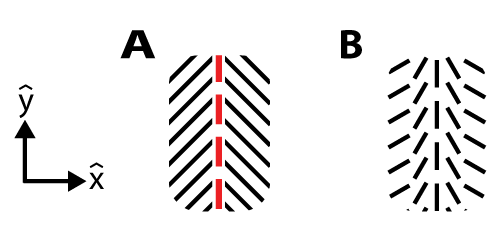
\includegraphics{figures/C2/Ch2-Figs_Smearing.png}
  \caption{Singular line defects are topologically unstable in 2D.
  (A) a singular line defect in 2D, with the singular region denoted in red.
  (B) A nonsingular structure resulting from a continuous deformation of (A).}\label{f:2-Smearing}
\end{figure}

Now, we consider a nematic in 3D.
Immediately, we see that the order parameter space is no longer $\mathbb{R}\mathbb{P}^1$, but instead is $\mathbb{R}\mathbb{P}^2$, the unit 2-sphere $\mathbb{S}^2$ with antipodal points identified, as we now need 2 angles to characterize all the possible orientations of $\mathbf{n}$~\cite{RN196,RN153,RN236}.
Another way to visualize $\mathbb{R}\mathbb{P}^2$ is as a hemisphere where only the base has antipodal points identified.
We first consider line defects with $d=1$ such that we characterize them with $\pi_{1}(\mathbb{R}\mathbb{P}^2)$, the fundamental group of $\mathbb{R}\mathbb{P}^2$.

Again, we consider $\mathbf{n}$ along a closed 1D contour in real space and the associated 1D contour in $\mathbb{R}\mathbb{P}^2$, with the topological charge given by the winding number.
However, we note that in $\mathbb{R}\mathbb{P}^2$, we can only have defects with $s =0,1/2$, as any contour on $\mathbb{R}\mathbb{P}^2$ with an integer value of $s$ can be continuously deformed into a point on $\mathbb{R}\mathbb{P}^2$ since ``you cannot lasso a sphere''~\cite{RN153}.
More explicitly, any contour on  $\mathbb{R}\mathbb{P}^2$ with integer $s$ must start and end at the same point.
Thus it can be ``slid'' to one side of the sphere and deformed to a point on $\mathbb{R}\mathbb{P}^2$, as illustrated schematically in Figure~\ref{f:2-RP2}(A,B).
This means that the only stable contours in $\mathbb{R}\mathbb{P}^2$ are those that start and end at antipodal points [see Figure~\ref{f:2-RP2}(C)], wrapping $\mathbb{R}\mathbb{P}^2$ exactly once.
This also means that contours starting and ending at the same point on $\mathbb{R}\mathbb{P}^2$ can be freely added and subtracted from a contour starting and ending at antipodal points on $\mathbb{R}\mathbb{P}^2$; thus, all contours starting and ending at antipodal points on $\mathbb{R}\mathbb{P}^2$ are homotopic.
Explicitly, this means that contours with $s = -1/2$ are homotopic to contours with $s = 1/2$ such that $\pi_1(\mathbb{R}\mathbb{P}^2)$ has only one nontrivial element, resulting in $s \in \{ 0,1/2\}$~\cite{RN153}.
As with walls in 3D and lines in 2D, this does not mean that $s = +1$ structures in 3D are impossible to create, it only means that they are not topologically stable structures and thus can only be stabilized by energetics.
Similarly, since an $s = -1/2$ line and an $s = +1/2$ line are homotopic, preferentially generating one structure over the other is a matter of tuning the free energy of each structure.
\begin{figure}
  \centering
  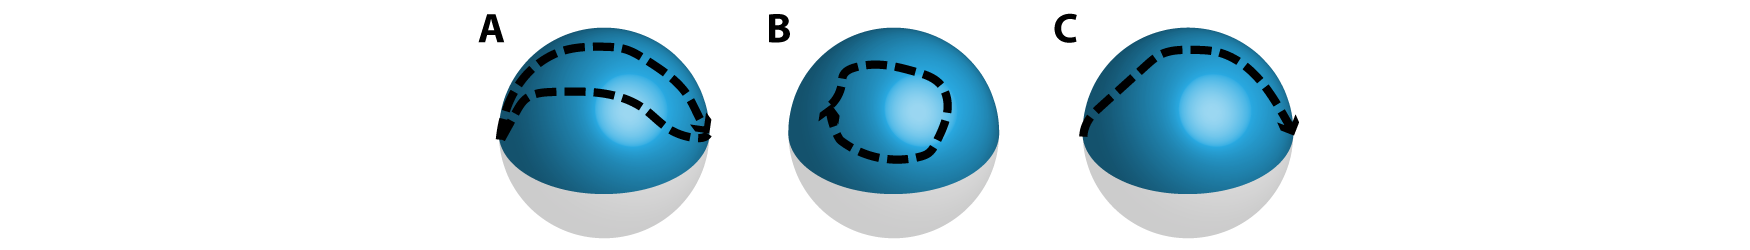
\includegraphics{figures/C2/Ch2-Figs_RP2.png}
  \caption{Contours in $\mathbb{RP}^2$.
  (A--C), Schematics showing $\mathbb{RP}^2$ (blue hemisphere) as $\mathbb{S}^2$ (full sphere) with antipodal points identified.
  A (A) contour that wraps $\mathbb{RP}^2$ twice can be (B) slid off and is homotopic to a point.
  A (C) contour that starts and ends at antipodal points is not homotopic to a point and is the only nontrivial contour in $\mathbb{RP}^2$.}\label{f:2-RP2}
\end{figure}

We lastly consider point defects in 3D characterized by the second homotopy group of $\mathbb{R}\mathbb{P}^2$, $\pi_{2}(\mathbb{R}\mathbb{P}^2)$.
Now, instead of mapping 1D closed contours in real space to $\mathbb{R}\mathbb{P}^1$ and $\mathbb{R}\mathbb{P}^2$ as we did with the fundamental group, we map a topologically spherical surface enclosing the defect to $\mathbb{R}\mathbb{P}^2$~\cite{RN196,RN153,RN236}.
In real space, we restate Eq.~\ref{e:1-HedgehogCharge} and calculate the topological ``hedgehog charge'' of a defect as~\cite{RN153}:
\begin{equation}
  q = \frac{1}{4 \pi} \oint_{\partial V} \textrm{d} \theta \, \textrm{d} \phi \, \mathbf{n} \cdot \left [ \partial_{\theta} \mathbf{n} \times \partial_{\phi} \mathbf{n} \right ],\label{e:2-hedCharge}
\end{equation}
 where $\theta$ and $\phi$ are the polar and azimuthal spherical angles, respectively, and $\partial V$ is the bounding surface of the closed volume $V$ containing the defect.
The volume $V$ must be homotopic to a sphere and thus can have no holes or handles.
From Chapter~\ref{c:1}, we know that this means that the Euler characteristic of $V$ is $\chi = 2$.
Physically, $q$ relates the orientations of $\mathbf{n}$ taken on a topologically spherical surface enclosing the defect to the number of times the orientations cover $\mathbb{S}^2$~\cite{RN153}.
Hedgehog charge is additive such that calculating $q$ for a volume containing only a $+q$ point defect and $-q$ point defect charge will yield $q_{net} = 0$.
Thus, $\pi_{2}(\mathbb{R}\mathbb{P}^2) = (\mathbb{Z}, +)$, the Abelian group consisting of the integers under addition.

It is important to note that there are 2 possible ways to turn a given director field into a vector field; either we take the vectors as $\mathbf{n}$ or as -$\mathbf{n}$.
Since we measure the hedgehog charge by considering how $\mathbf{n}$ on a surface homeomorphic to $\mathbb{S}^2$ covers $\mathbf{RP}^2$, this ambiguity means that any defect in isolation can only be determined up to $|q|$~\cite{RN153}.
Thus, while topological character is determined by homotopy theory, the sign of charge can only be determined relative to a \emph{basepoint} defining the projection from $\mathbb{R}\mathbb{P}^2$ to $\mathbb{S}^2$~\cite{RN153}.
For example, the defect structures drawn schematically in Figure~\ref{f:2-3DMeas}(A,B) cannot be distinguished \emph{a priori} in order parameter space.
However, if we choose a basepoint such that the structure in Figure~\ref{f:2-3DMeas}(A) has $q = +1$, evaluating the structure in Figure~\ref{f:2-3DMeas}(B) under the same basepoint will yield $q = -1$.
We will keep this basepoint for the remainder of the Thesis.
\begin{figure}[h]
  \centering
  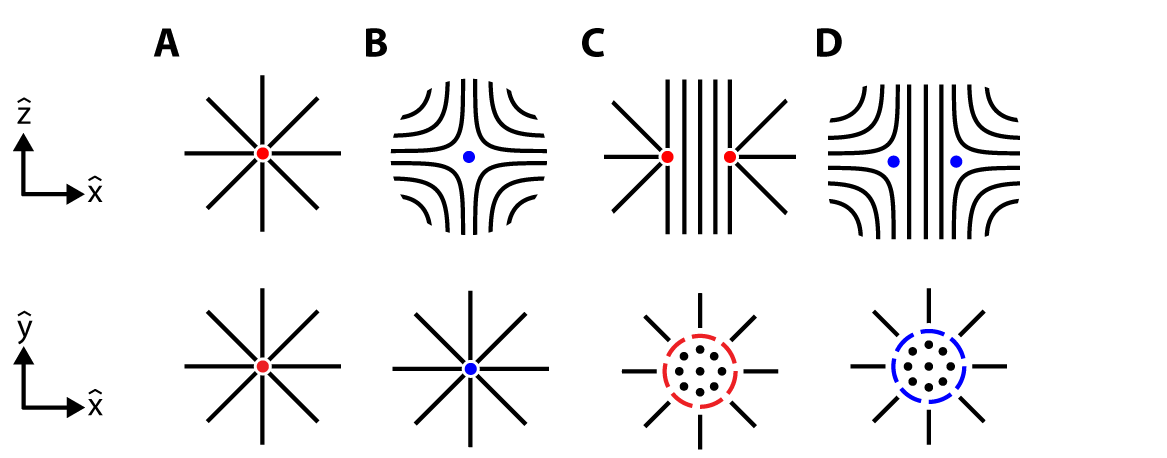
\includegraphics{figures/C2/Ch2-Figs_3DMeas.png}
  \caption{Examples of defect structures in 3D.
  (A-D), Cross sections in the $xz$ and $xy$ planes of defect structures with $|q| = 1$.
  Once we choose a reference point that defines the projection of $\mathbf{n}$ onto the unit sphere, we can distinguish the structures in A,C from the structures in B,D.
  Without loss of generality, we take the convention that the structures in A,C have $q = +1$ such that the structures in B,D have $q = -1$.
  (A,B), schematics of a (A) radial and a (B) hyperbolic hedgehog defect.
  (C,D), schematics of a (C) radial ring and a (D) hyperbolic ring defect.
  Note that the ring defects in (C,D) are formed by an $s = +1/2 $ and an $s = -1/2$ line defect that has closed in on itself.}\label{f:2-3DMeas}
\end{figure}

Similar to how additivity means that a volume enclosing a $+q$ point defect and $-q$ point defect charge will yield $q_{net} = 0$, the point defect structures in Figure~\ref{f:2-3DMeas}(A,B) are not the only structures with $|q| = 1$.
In fact, ring defects, as depicted schematically in Figure~\ref{f:2-3DMeas}(C,D) are homotopic to their respective point defect counterparts in Figure~\ref{f:2-3DMeas}(A,B).
Shrinking the ring radius of the radial ring in Figure~\ref{f:2-3DMeas}(C) yields the radial hedgehog shown in Figure~\ref{f:2-3DMeas}(A) and shrinking the ring radius in the hyperbolic ring in Figure~\ref{f:2-3DMeas}(D) yields a hyperbolic hedgehog like the one shown in Figure~\ref{f:2-3DMeas}(B).
A ring defect can be thought of as a line defect in 3D [see Figure~\ref{f:2-GenDef}] that is bent into a circle.
Hence, if we were to draw a closed 1D contour that passed through the ring and ``linked'' with the ring defect, we would find that radial rings with $q = +1$ are formed with $s = +1/2$ lines and hyperbolic rings with $q = -1$ are formed with $s = -1/2$ lines.

Finally, we briefly want to touch on the use of the term ``charge'' to characterize defects in NLC.\@
The choice of this term is no accident and reflects an analogy with electric charges.
This analogy is born out not only in the additivity of both defect charges and electric charges, but also in their pairwise interactions~\cite{RN33,RN175,RN207}.
Recall from Eq.~\ref{e:1-TopTheoryofDefects} that the free energy of a nematic configuration with defects on a surface has the exact form of the free energy of a plasma, where the defects act like the charges in the plasma.
Defects in 2D and 3D with like-signed charge repel and defects with opposite-signed charge attract and even annihilate.




\section{Frank-Oseen free energy}
Since the constituent particles, or mesogens, in a nematic material prefer to align along the $\mathbf{n}$, the ideal state for a nematic phase is a homogeneously-aligned state with $\mathbf{n}$ a constant everywhere.
Distortions from this uniform state cost energy.
Since in most experiments the director distortions occur over much larger length scales than the length of the mesogens --- $|\nabla \mathbf{n}| a \ll 1$, where $a$ is the mesogen length --- we can bypass the behavior of individual mesogens and instead use a continuum model for the free energy density that depends on $\mathbf{n}$ only.
Here, we follow the work of F.C. Frank~\cite{RN61} and expand about the undistorted director state in powers of $|\nabla \mathbf{n}|$.
This is a phenomenological approach similar to Hooke's elasticity theory of a solid~\cite{RN175,RN178}; however, instead of focusing on restoring stresses that oppose strains, we look for restoring torques that oppose curvature-strains in the director field.
This is again a reflection that there is no restriction to the center-of-mass positions of the mesogens; the nematic elasticity only opposes deformations in the orientations of the mesogens.

\subsection{A brief derivation}
Let a local coordinate system at a point be defined by $\{x_1, x_2, x_3 \}$ such that we can define $\mathbf{n} = (\mathbf{n} \cdot \hat{e}_i) \hat{e}_i = n_i$, where we again sum over repeated indices, and $\hat{e}_i$ is the unit vector associated with $x_i$ and $\{\hat{e}_1, \hat{e}_2, \hat{e}_3 \}$ forms an orthonormal basis.
If we let $\hat{e}_3$ be parallel to $\mathbf{n}$ at the point and consider situations where $x_i \ll 1$, we can locally expand $n_i$ as:
\begin{align}
  n_1 &= \frac{\partial n_1}{\partial x_1}x_1 + \frac{\partial n_1}{\partial x_2}x_2 + \frac{\partial n_1}{\partial x_3}x_3 + \mathcal{O}\big (x^2 \big ) \nonumber \\
      &= a_1 x_1 + a_2 x_2 + a_3 x_3 + \mathcal{O}\big (x^2 \big )\label{e:2-LocalCoordA}  \\
  n_2 &= \frac{\partial n_2}{\partial x_1}x_1 + \frac{\partial n_2}{\partial x_2}x_2 + \frac{\partial n_2}{\partial x_3}x_3 + \mathcal{O}\big (x^2 \big ) \nonumber  \\
      &= a_4 x_1 + a_5 x_2 + a_6 x_3 + \mathcal{O}\big (x^2 \big )\label{e:2-LocalCoordB}  \\
  n_3 &= 1 + \mathcal{O}\big (x^2 \big ). \nonumber
\end{align}
Now expanding about the undistorted state, we can write the free energy density to quadratic order in the first derivatives as:
\begin{equation}
  f(\mathbf{n}) = K_i a_i + K_{ij} a_i a_j,\label{e:2-FrankGeneralExpansion}
\end{equation}
where $i,j = \{ 1,2 \dots, 6 \}$, giving us 42 possible terms.
However, any free energy must respect the symmetry of the nematic phase and be invariant under exchange of $i$ and $j$, invariant under inversion of $\mathbf{n} \rightarrow -\mathbf{n}$, invariant under arbitrary rotations about $\mathbf{n}$, and invariant with respect to the handedness of the coordinate system~\cite{RN61}.
Under these conditions, all of the 6 $K_i$ terms vanish and of the 36 terms in $K_{ij}$, 26 vanish and only 4 are independent, giving the coefficient matrix:
\begin{equation}
  K_{ij} =
  \begin{pmatrix}
    K_{11} & 0 & 0 & 0 & (K_{11}-K_{22}-K_{24}) & 0 \\
    0 & K_{22} & 0 & K_{24} & 0 & 0 \\
    0 & 0 & K_{33} & 0 & 0 & 0 \\
    0 & K_{24} & 0 & K_{22} & 0 & 0 \\
    (K_{11}-K_{22}-K_{24}) & 0 & 0 & 0 & K_{11} & 0 \\
    0 & 0 & 0 & 0 & 0 & K_{33} \\
  \end{pmatrix}.\label{e:2-Kijreduced}
\end{equation}
Substituting Eq.~\ref{e:2-Kijreduced} into Eq.~\ref{e:2-FrankGeneralExpansion} and collecting terms, we are left with the expression:
\begin{align}
  f(\mathbf{n}) = \frac{1}{2}K_{11} (a_1 + a_5)^2 + \frac{1}{2}&K_{22} (a_2 - a_4)^2 + \frac{1}{2}K_{33} (a_3^2 + a_6^2) \nonumber \\
    &- (K_{22} + K_{24}) (a_1 a_5 - a_2 a_4).\label{e:2-FrankLocalExpansion}
\end{align}
If we return to the source of the $a_i$ coefficients in Eqs.~\ref{e:2-LocalCoordA}, \ref{e:2-LocalCoordB}, we can uncover the physical significance of the distortions:
\begin{align}
  s_1 = a_1 = \frac{\partial n_1}{\partial x_1} \quad & \quad s_2 = a_5 = \frac{\partial n_2}{\partial x_2}\label{e:2-PhysicalDistortionsA} \\
  t_1 = - a_4 = -\frac{\partial n_2}{\partial x_1} \quad & \quad t_2 = a_2 = \frac{\partial n_1}{\partial x_2}\label{e:2-PhysicalDistortionsB} \\
  b_1 =  a_3 = \frac{\partial n_1}{\partial x_3} \quad & \quad b_2 = a_6 = \frac{\partial n_2}{\partial x_3},\label{e:2-PhysicalDistortionsC}
\end{align}
where we have renamed the coefficients to reflect their associated distortion, with $s_1$ and $s_2$ signifying a ``splay'' distortion, $t_1$ and $t_2$ signifying a ``twist'' distortion, and $b_1$ and $b_2$ signifying a ``bend'' distortion.
These distortions in the local frame are easily visualized, as seen in Figure~\ref{f:2-FrankDist}(A--C), respectively.
Now if we use Eqs.~\ref{e:2-PhysicalDistortionsA}--\ref{e:2-PhysicalDistortionsC} to re-write Eq.~\ref{e:2-FrankLocalExpansion}, we have:
\begin{align}
  f(\mathbf{n}) = \frac{1}{2}K_{11} (s_1 + s_2)^2 + \frac{1}{2}&K_{22} (t_1 + t_2)^2 + \frac{1}{2}K_{33} (b_1^2 + b_2^2) \nonumber \\
    & - (K_{22} + K_{24}) (s_1 s_2 + t_1 t_2).\label{e:2-FrankPhysicalExpansion}
\end{align}

\begin{figure}
  \centering
  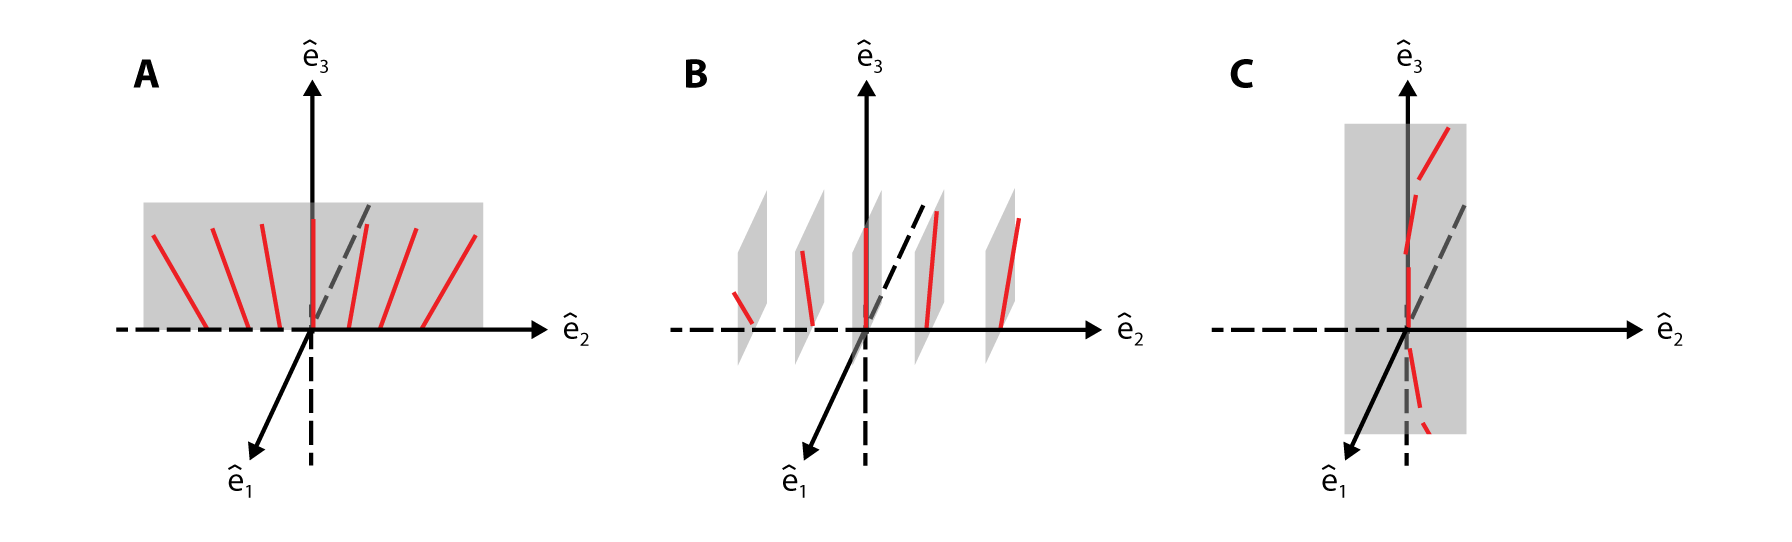
\includegraphics{figures/C2/Ch2-Figs_FrankDist.png}
  \caption{Nematic distortions in the local frame. (A), A schematic showing a splay distortion corresponding to a nonzero $s_2$.
  (B), A schematic showing a twist distortion corresponding to a nonzero $t_2$.
  (C), A schematic showing a bend distortion corresponding to a nonzero $b_2$.}\label{f:2-FrankDist}
\end{figure}
Hence, we see that each term in the free energy density comes from a different distortion, such that the elastic constants $K_{ij}$ hold the relative importance of each distortion for a given material.
For example, consider a NLC with $K_{11} \gg K_{33} = K_{22} = K_{24}$; under confinement or strain, this material will prefer to bend and twist instead of splay.
The elastic constants are named after their associated distortion, with $K_{11}$ known as the splay elastic constant, $K_{22}$ the twist elastic constant, $K_{33}$ the bend elastic constant, and $K_{24}$ the saddle-splay elastic constant.
Note that the saddle-splay distortion is unique as it is associated with both the twist elastic constant and the saddle-splay elastic constant.

The ability to associate individual distortions with their elastic constant gives the Frank-Oseen free energy incredible intuitive power; it is easy to visualize each distortion's contribution to the director field.
Finally, we can recast the distortions in Eq.~\ref{e:2-FrankLocalExpansion} in terms of standard vector calculus operations, arriving at the well-known expression for the Frank-Oseen Free Energy~\cite{RN61}:
\begin{align}
  f(\mathbf{n}) = \frac{1}{2}K_{11} (\nabla \cdot \mathbf{n})^2 + \frac{1}{2}&K_{22} (\mathbf{n} \cdot \nabla \times \mathbf{n})^2 + \frac{1}{2}K_{33} (\mathbf{n} \times \nabla \times \mathbf{n})^2 \nonumber \\
    & - \frac{1}{2}(K_{22} + K_{24}) \nabla \cdot (\mathbf{n}\nabla \cdot \mathbf{n} + \mathbf{n} \times \nabla \times \mathbf{n}).\label{e:2-FrankFinalExpansion}
\end{align}

Note that while Frank pioneered the phenomenological approach for a liquid crystalline free energy, his was not the first attempt to construct a free energy for liquid crytals.
Oseen arrived at a similar expression to Eq.~\ref{e:2-FrankFinalExpansion} before Frank, but he approached the problem from a microscopic approach under the assumption that the free energy could be calculated considering interactions between all possible pairs of molecules~\cite{RN205}.
While Oseen's final expression for a nematic misses some of the terms in Eq.~\ref{e:2-FrankFinalExpansion}, it is close enough that Eq.~\ref{e:2-FrankFinalExpansion} carries the names of both Frank and Oseen.


\subsection{Nehring, Saupe, and second derivatives}
We arrived at Eq.~\ref{e:2-FrankFinalExpansion} by expanding about the undistorted state to quadratic order in powers of the 1$^\textup{\rm st}$ derivatives of $\mathbf{n}$.
Due to the symmetry of the nematic, all of the terms linear in $|\nabla \mathbf{n}|$ vanished, making the quadratic terms the lowest order surviving terms in the expansion.
However, as Nehring and Saupe pointed out, a full expansion to the lowest order should also include 2$^\textup{\rm nd}$ derivatives of $\mathbf{n}$ as they can contribute to the Frank-Oseen free energy at order $\mathcal{O}(x^2)$ as well~\cite{RN60}.
In fact, Oseen's original free energy expression also included terms depending on 2$^\textup{\rm nd}$ derivatives of $\mathbf{n}$ that Frank neglected~\cite{RN205}.
Thus, Eq.~\ref{e:2-FrankGeneralExpansion} becomes:
\begin{equation}
  f(\mathbf{n}) = K_i a_i + K_{ij} a_i a_j + K'_{ij} a_{i,j},\label{e:2-NSGeneralExpansion}
\end{equation}
where $a_{i,j}$ represents $\dfrac{\partial a_i}{\partial x_j}$, giving us 18 terms in the $K'_{ij}$ coefficient matrix.
Again using the symmetries of a nematic, collecting terms, and rewriting the expression in terms of vector calculus manipulations, we arrive at a new expression for the free energy:
\begin{align}
  f(\mathbf{n}) = \frac{1}{2}&(K_{11} - 2K'_{13}) (\nabla \cdot \mathbf{n})^2 + \frac{1}{2}K_{22} (\mathbf{n} \cdot \nabla \times \mathbf{n})^2 + \frac{1}{2}(K_{33} + 2K'_{13}) (\mathbf{n} \times \nabla \times \mathbf{n})^2 \nonumber \\
    & - \frac{1}{2}(K_{22} + K_{24}) \nabla \cdot (\mathbf{n}\nabla \cdot \mathbf{n} + \mathbf{n} \times \nabla \times \mathbf{n})
      + K'_{13} \nabla \cdot (\mathbf{n} \nabla \cdot \mathbf{n}),\label{e:2-NSFinalExpansion}
\end{align}
where we see that the elastic constants associated with splay and bend are renormalized by $K'_{13}$, and that a new term called ``splay-bend'' associated with the distortion $\nabla \cdot (\mathbf{n} \nabla \cdot \mathbf{n})$ has appeared~\cite{RN60}. \\

Since Eqs~\ref{e:2-FrankFinalExpansion} and~\ref{e:2-NSFinalExpansion} are phenomenological expressions, renormalizing the splay and bend elastic constants doesn't affect underlying physics.
This leaves the addition of the splay-bend term as the most significant effect of considering 2$^\textup{\rm nd}$ order derivatives of $\mathbf{n}$.
The splay-bend term itself is subject to controversy as its inclusion to the free energy makes the free energy unbounded from below~\cite{RN214,RN215,RN216}.
We follow Ref.~\cite{RN219} and illustrate this with a simple example of a NLC confined between two parallel plates.
Let one plate be at $z = 0$ and the other at $z=d$, and let the director vary only in the $xz$-plane.
We can then write our director in terms the angle $\phi$ in the $xz$-plane measured off of the $x$-axis.
Let the director field have the form $\phi_n(z) = \phi_d + \beta ((z/d)^n-1)$, such that $\phi(0) = \phi_d - \beta$ and $\phi(d) = \phi_d$, with $\phi_d$ and $\beta$ fixed angles that give the boundary conditions.
In this case, $n$ is a positive integer that governs how the director varies between the two plates.
This geometry is known as the splay-bend geometry.
For simplicity, we take $K_{11} = K_{33} = K$, and assume $n$ is large, allowing us to approximate the free-energy as
\begin{align}
  F &= \frac{1}{4}\frac{K \beta^2}{d^2}n + \frac{K_{13} \sin (2 \phi_d)\beta}{2d}n \\
  &= \frac{1}{4}\frac{K \beta^2}{d^2} \left ( 1 + \frac{2 K_{13} \sin(2 \phi_d)}{K \beta}  \right) n.\label{e:2-UnboundedFromBelow}
\end{align}
If we require $\beta < -2 K_{13} \sin(2 \phi_d) /K$ and $\phi_d \neq 0, \pi/2$, we see that the \\ $1 + 2 K_{13} \sin(2 \phi_d)/(K \beta) $ term in Eq.~\ref{e:2-UnboundedFromBelow} is negative, and
\begin{align}
  \lim_{n\to\infty} &F = -\infty, \\
  \lim_{n\to\infty} &\phi_n(z) =
  \begin{cases}
    \phi(d) - \beta \quad \textrm{if }  0 \leq z  < d \\
    \phi_d \quad \textrm{if} z = d.
  \end{cases}
\end{align}
Here, we see that that our director field has a free energy that diverges to $- \infty$, leading to a discontinuity in our director field.
The discontinuity is called the Oldano-Barbero discontinuity.
Recall that we initially derived the Frank-Oseen free energy assuming small deformations --- however, we have just shown a situation where the Frank-Oseen free energy diverges and leads to a discontinuity in the director field.
This situation is called the Oldano-Barbero paradox~\cite{RN216,RN220,RN219,RN221}.\fxnote{check the FE expression}

The easiest way to solve the paradox is to set $K_{13} = 0$.
It is worth noting that there has been a concerted effort to solve the paradox without setting $K_{13} = 0$~\cite{RN220,RN221,RN55,RN222}.
However, careful experiments in the splay-bend geometry have found $K_{13} = 0$ within the experimental error, and the experimenters never observe a discontinuity in the director field~\cite{RN312}.
Consequently, the most common approach is to neglect the splay-bend term altogether~\cite{RN55,RN222}.


\subsection{Insights from microscopic calculations}
There has been significant theoretical effort, starting with the pioneering work of Oseen, to relate the microscopic interactions between the nematic mesogens to the macroscopic, measurable $K_{ij}$ of the nematic phase~\cite{RN56,RN55,RN205,RN217,RN225,RN224,RN218,RN222}.
While an in-depth discussion of the various methods and results is beyond the scope of this document, it is worthwhile to examine the general process and consider the implications for the $K_{ij}$ in the phenomenological expressions derived earlier.
At the most basic level, the total interaction energy for a system is the sum over the pairwise interaction energy for all pairs of mesogens in the system.
% Since the interaction potential is positive definite, we see from the microscopics that any elastic constant in Eq~\ref{e:2-FrankFinalExpansion} or Eq.~\ref{e:2-NSFinalExpansion} must be greater than or equal to 0~\cite{RN205}.

However, an energy constructed upon the physical mesogens themselves requires us to know the position and orientation of each individual mesogen.
Thus, it is common to consider instead the particle density as a function of orientation and position and integrate over all possible pairs of points in the volume~\cite{RN222}.
This is a density functional theoretic approach~\cite{RN223} and thus yields an energy similar to the general expression~\cite{RN56,RN55}:
\begin{equation}
  F = \int \textrm{d}\mathbf{R} \textrm{d}\mathbf{R}' \, G(\mathbf{R},\mathbf{R}'),
\end{equation}
where $\mathbf{R}$ and $\mathbf{R}'$ are positions, and $G(\mathbf{R},\mathbf{R}')$ is an interaction energy density satisfying $G(\mathbf{R},\mathbf{R}') = 0$ for $|\mathbf{R}-\mathbf{R}'| \gg 0$, reflecting the finite interaction range between the mesogens.
However, we are looking for a free energy and not just the interaction energy of the system.
Thus, it is common to calculate the energy for a homogeneous state and then expand about the homogeneous state to get an expression for a distortion free energy; this is similar to how we derived the Frank-Oseen free energy earlier.
Since we are looking to derive an expression for the free energy as a functional of director field, we must satisfy
\begin{equation}
  F = \int \textrm{d}\mathbf{R} \textrm{d}\mathbf{R}' \, G(\mathbf{R},\mathbf{R}')
  = \int \textrm{d} \mathbf{r} \, f(\mathbf{r}),\label{e:2-NonlocalLocal}
\end{equation}
where $f(\mathbf{r})$ is a function of position, $\mathbf{r}$.
Note that there is not a unique relation between $f(\mathbf{r})$ and $G(\mathbf{R},\mathbf{R}')$; more specifically, $f$ will be determined by how we choose $r$.
For example, if $\mathbf{r} = \mathbf{R}$, then $f(\mathbf{r}) = \int \textrm{d}\mathbf{R}' \, G(\mathbf{r},\mathbf{R}')$.
However, if $\mathbf{r} = (\mathbf{R} + \mathbf{R}')/2$, then $f(\mathbf{r}) = \int \textrm{d}\mathbf{R}' \, G(2\mathbf{r} - \mathbf{R}',\mathbf{R}')$.
Since there are an infinite number of possibilities to choose $\mathbf{r}$ and thus determine $f$, any elastic constants in $f(\mathbf{r})$ cannot depend on how we choose $\mathbf{r}$~\cite{RN55}.
In addition, the microscopic calculations are performed with a density function that is dependent on position and orientation, $\rho(\mathbf{r},\mathbf{\omega})$, where $\mathbf{\omega}$ specifies an orientation; however, the phenomenological free energy expressions are only a function of the director field.
% Thus, we must also satisfy:
% \begin{equation}
%   F[\mathbf{n}] = \int \textrm{d} \mathbf{r} \, f(\mathbf{n}) = \int \textrm{d} \mathbf{r} \, f \big ( \rho(\mathbf{r},\mathbf{\omega}) \big),\label{e:2-LessInfo}
% \end{equation}
% where $\mathbf{n}$ is a function of $\mathbf{r}$.
% Since the director contains less information than the complete density function, in general there is not a unique way to determine $\mathbf{n}(\mathbf{r})$ from $\rho(\mathbf{r},\mathbf{\omega})$~\cite{RN55}.
% For a distortion of wavelength $\xi$ and amplitude $\epsilon$, we can only uniquely determine $\mathbf{n}(\mathbf{r})$ if we restrict ourselves to the lowest energy distortions in the long-wavelength $(\xi \rightarrow \infty)$ and small amplitude $(\epsilon \ll 1)$ regime.
% These modes come from the Nambu-Goldstone theorem, which requires that any broken continuous symmetry results in a soft mode, i.e.\ a mode whose distortion cost vanishes as $\xi^{-2}$ and whose susceptibility diverges in the limit $\xi \rightarrow \infty$~\cite{RN175,RN226,RN227,RN228}.
% These soft modes are the weakest modes possible and thus will define the leading order in the free energy, making the free energy a unique functional of $\mathbf{n}$~\cite{RN55}. \\

Given this condition, microscopic calculations show that $K_{11}$, $K_{22}$, $K_{33}$, and $K_{24}$ are real physical material properties~\cite{RN55,RN56,RN225,RN224,RN217,RN222}.
However, $K'_{13}$ depends on the choice of $\mathbf{r}$, and therefore cannot be a real material parameter.
% Consequently, $K'_{13} = 0$~\cite{RN55,RN225}.
% The conclusion that $K'_{13} = 0$ also holds when calculations are done close to a boundary provided the $\mathbf{n} = -\mathbf{n}$ inversion symmetry is maintained~\cite{RN56}.
% Since inversion symmetry is assumed in deriving the phenomenological expressions in Eqs.~\ref{e:2-NSFinalExpansion} and~\ref{e:2-FrankFinalExpansion}, situations that violate inversion symmetry create far more issues than simply the inclusion of a $K_{13}'$ term.
% Note that while there have been microscopic calculations that predict a nontrivial $K'_{13}$, these calculations~\cite{RN224,RN217,RN222} have specified a $(\mathbf{R},\mathbf{R}') \rightarrow \mathbf{r}$ mapping, rendering their $K'_{13}$ values invalid.
Thus, the Oldano-Barbero paradox is resolved and the common approach of neglecting splay-bend is valid.
With $K_{13}'=0$, we see that Eq.~\ref{e:2-NSFinalExpansion} reduces to the expression for the Frank-Oseen free energy in Eq.~\ref{e:2-FrankFinalExpansion}.

Microscopic calculations also show that close to a boundary, $K_{ij}$ in general deviate from their bulk values and become position-dependent.
This is because the mesogens are now interacting with the material outside of the nematic volume~\cite{RN56,RN57,RN55}.
However, this interaction is limited by the range of the intermolecular potential, such that the position dependence of the $K_{ij}$ vanishes over a small boundary layer --- beyond this layer the $K_{ij}$ return to their bulk values, which depend only on the specific nematic material.
In summary, microscopic calculations show that the free energy of a NLC is composed of terms quadratic in $|\nabla \mathbf{n}|$.
Even though terms linear in $|\nabla ^2 \mathbf{n}|$ could in principle contribute to the free energy to the same order as terms quadratic in the 1$^\textup{\rm st}$ derivatives, microscopic calculations show that the coefficients associated with 2$^\textup{\rm nd}$-derivative distortions vanish, thus removing the problems that the 2$^\textup{\rm nd}$-derivative distortions bring.
% In addition, since the free energy is constructed using a positive-definite pairwise potential, all the elastic constants in the phenomenological free energy expressions must be greater than or equal to 0.


\subsection{Saddle-splay and curvature-coupling}
If we take a look at the terms in the Frank-Oseen free energy in Eq.~\ref{e:2-FrankFinalExpansion}, we can see a difference between the saddle-splay term and the splay, twist, and bend terms.
Notice that since all the $K_{ij} \geq 0$, the energetic cost of splay, bend, and twist distortions are positive semi-definite.
In contrast, the saddle-splay distortion can be either positive or negative.
In addition, the saddle-splay distortion is the divergence of a vector, giving us the option of re-writing the distortion in terms of a surface integral using the divergence theorem~\cite{RN230}:
\begin{align}
  F_{24}[\mathbf{n}] &= - \frac{1}{2}\int_{V} \textup{d}^3  \mathbf{r} \bigg \{ (K_{22} + K_{24})  \nabla \cdot (\mathbf{n}\nabla \cdot \mathbf{n} + \mathbf{n} \times \nabla \times \mathbf{n}) \bigg \}\label{e:2-F24GaussA}  \\ &=
  - \frac{1}{2}(K_{22} + K_{24}) \oint_{\partial V} \textup{d}^2  \mathbf{r} \bigg \{   \mathbf{k} \cdot (\mathbf{n}\nabla \cdot \mathbf{n} + \mathbf{n} \times \nabla \times \mathbf{n}) \bigg \},\label{e:2-F24GaussB}
\end{align}
where $V$ is a volume, $\partial V$ is a piecewise-smooth manifold bounding $V$, and $\mathbf{k}$ is the unit surface normal.

Note that the $\mathbf{n}$ needs to be continuous and differentiable everywhere on $\partial V$, meaning that the manifold needs to be defect-free.
However, since $\partial V$ only needs to be piecewise continuous, we can always draw the manifold to exclude any defects.
Therefore, the divergence theorem can always be applied, implying that any nontrivial saddle-splay distortion in $V$ must affect $\mathbf{n}$ on $\partial V$.
In contrast, nontrivial splay, bend, and twist distortions can exist purely in the bulk, such that $\mathbf{n}$ is affected in $V$ but not on $\partial V$.
In fact, the ability to generate pure bulk distortions for splay, twist, and bend allow for easy measurements of $K_{ij}$ via the Freederickz transition, for example~\cite{RN212,RN213,RN33,RN188,RN182,RN183}.
In these measurements, the bulk volume is always large enough such that any contribution from the position-dependence of $K_{ij}$ near the boundaries is negligible.

Due to the connection between the bulk saddle-splay distortion and the director orientation on a bounding manifold, the saddle-splay distortion term is often referred to as a surface-like term and sometimes even referred to as an effective anchoring term~\cite{RN206,RN33,RN194,RN58,RN57,RN151}.
Since any measurement of $K_{24}$ requires $\mathbf{n}$ to change at an interface, there is concern that the position-dependence of $K_{ij}$ near an interface leads to the inability to measure the bulk value of $K_{24}$ without contamination from the interface.
However, we emphasize that while it is tempting to treat $F_{24}$ as a surface term where the energy cost is calculated using the value of $K_{ij}$ at the interface like,
\begin{equation}
  F_{24}[\mathbf{n}] = - \frac{1}{2}(K_{22}(\mathbf{r}) + K_{24}(\mathbf{r}))_{\mathbf{r} \rightarrow \partial V} \oint_{\partial V} \textup{d}^2  \mathbf{r} \bigg \{   \mathbf{k} \cdot (\mathbf{n}\nabla \cdot \mathbf{n} + \mathbf{n} \times \nabla \times \mathbf{n}) \bigg \},
\end{equation}
this is incorrect.
The divergence theorem cannot be used if $K_{ij}$ is position-dependent since the integrand in Eq.~\ref{e:2-F24GaussA} is no longer the divergence of a vector.
In fact, measuring $K_{24}$ is in principle no different than measuring any of the $K_{ii}$ --- provided the volume of the bulk is much larger than the boundary layer, the influence of the position-dependence of $K_{ij}$ is negligible.

To demonstrate this, we return to Eq.~\ref{e:2-F24GaussA} and insert the position-dependence:
\begin{equation}
  F_{24} = -\frac{1}{2}\int_{V}\textup{d}^3\mathbf{r} \left \{ (K_{22} (\mathbf{r}) + K_{24}(\mathbf{r})) \nabla \cdot (\mathbf{n} \nabla \cdot \mathbf{n} + \mathbf{n} \times \nabla \times \mathbf{n}) \right \}.\label{e:2-F24GaussPosition}
\end{equation}
Integrating Eq.~\ref{e:2-F24GaussPosition} by parts with $\mathbf{A}(\mathbf{r}) = \mathbf{n} \nabla \cdot \mathbf{n} + \mathbf{n} \times \nabla \times \mathbf{n}$, \newline $K_*(\mathbf{r}) = -(K_{22} (\mathbf{r}) + K_{24}(\mathbf{r})/2)$, and $\bm{\alpha}$ describing the boundary yields:
\begin{align}
  \int_{V}\textup{d}^3\mathbf{r} \left \{ K_{*} (\mathbf{r}) \nabla \cdot \mathbf{A} \right \} &=
  \oint_{\partial V}\textup{d}^2 \mathbf{r} \left \{ \mathbf{k} \cdot (K_{*} (\bm{\alpha}) \mathbf{A}(\bm{\alpha}) \right \} -  \int_{V} \textup{d}^3\mathbf{r} \left \{ \mathbf{A} \cdot \nabla K_{*} (\mathbf{r}) \right \}  \\ &=
  K_*(\bm{\alpha}) \oint_{\partial V} \textup{d}^2\mathbf{r} \left \{ \mathbf{k} \cdot \mathbf{A}(\bm{\alpha})\right \} - \int_{V} \textup{d}^3\mathbf{r} \left \{ \mathbf{A} \cdot \nabla K_{*} (\mathbf{r}) \right \}, \label{e:2-pos_stokes1}
\end{align}
where we have chosen $\mathbf{k}$ as the outward-pointing unit normal and we have pulled $K_*(\partial V)$ out of the integral as $K_*$ only depends on the distance from the boundary~\cite{RN55}.
Now, we separate $K_*(\mathbf{r}) = K_* + K_*^s(\mathbf{r})$ into the bulk material constant $K_*$ and the position-dependent contribution $K_*^s(\mathbf{r})$, where $K_*^s(\mathbf{r})$ decays across a boundary layer of thickness $d_l$.
Substituting this into Eq.~\ref{e:2-pos_stokes1}, we are left with:
\begin{align}
  \int_{V}\textup{d}^3\mathbf{r} \left \{ K_{*} (\mathbf{r}) \nabla \cdot \mathbf{A} \right \} &=
  (K_*+K_*^s(\bm{\alpha})) \oint_{\partial V} \textup{d}^2\mathbf{r} \left \{ \mathbf{k} \cdot \mathbf{A}(\bm{\alpha})\right \} \nonumber \\&
  \quad \quad - \int_{V} \textup{d}^3\mathbf{r} \left \{ \mathbf{A} \cdot \nabla K_{*}^s (\mathbf{r}) \right \}. \label{e:2-pos_stokes2}
\end{align}
If we now expand $\mathbf{A}(\mathbf{r})$ and $\nabla K_*^s(\mathbf{r})$ over the boundary layer with $\mathbf{r} = \bm{\alpha} - \zeta \mathbf{k}$, where $\zeta$ is the distance from the boundary, we have:
\begin{align}
  \mathbf{A}(\bm{\alpha} - \zeta \mathbf{k}) &\approx \mathbf{A}(\bm{\alpha}) - \zeta (\mathbf{k} \cdot \nabla \mathbf{A}(\bm{\alpha}))_{\zeta = 0} \label{e:2-expandA} \\
  \nabla K_*^s(\bm{\alpha} - \zeta \mathbf{k}) &\approx \mathbf{k} (\mathbf{k} \cdot \nabla K_*^s(\bm{\alpha} - \zeta \mathbf{k}))_{\zeta = 0} - \zeta\, \mathbf{k}(\mathbf{k} \cdot \nabla (\mathbf{k} \cdot \nabla K_*^s(\bm{\alpha} - \zeta \mathbf{k})))_{\zeta = 0}
\end{align}
As $K_*^s(\mathbf{r})$ decays across a boundary layer of thickness $d_l$, we can approximate the leading order term in $\nabla K_*^s(\bm{\alpha} - \zeta \mathbf{k})$ as:
\begin{equation}
  \mathbf{k} (\mathbf{k} \cdot \nabla K_*^s(\bm{\alpha}))_{\zeta = 0} =
  \begin{cases}
    \mathbf{k}\frac{K_*^s(\bm{\alpha})}{d_l} & 0 \leq \zeta \leq d_l \\
    0 & \textup{otherwise}
  \end{cases}
\end{equation}
Thus, to leading order we can write the 2$^\textrm{\rm nd}$ term in Eq.~\ref{e:2-pos_stokes2} as
\begin{align}
  \int_{V} \textup{d}^3\mathbf{r} \left \{ \mathbf{A} \cdot \nabla K_{*}^s (\mathbf{r}) \right \} & \approx
  \int_{V} \textup{d}^3\mathbf{r} \left \{\mathbf{A}(\bm{\alpha}) \cdot \mathbf{k}(\mathbf{k} \cdot \nabla K_*^s(\bm{\alpha}))  + \mathcal{O}(\zeta) \right \} \\ & \approx
  \mathbf{k} \cdot \nabla K_*^s(\bm{\alpha}) \int_{V} \textup{d}^3\mathbf{r}\left \{\mathbf{A}(\bm{\alpha}) \cdot \mathbf{k} + \mathcal{O}(\zeta) \right \} \\ & \approx
  \frac{K_*^s(\bm{\alpha})}{d_l} \oint_{\partial V} \textup{d}^2\mathbf{r}\left \{d_l\,\mathbf{A}(\bm{\alpha}) \cdot \mathbf{k} \right \} \\ & \approx
  K_*^s(\bm{\alpha}) \oint_{\partial V} \textup{d}^2\mathbf{r}\left \{ \mathbf{k}  \cdot \mathbf{A}(\bm{\alpha}) \right \} + \mathcal{O}(d_l^2).
\end{align}
Substituting back into Eq.~\ref{e:2-pos_stokes2}, we have:
\begin{equation}
  \int_{V}\textup{d}^3\mathbf{r} \left \{ K_{*} (\mathbf{r}) \nabla \cdot \mathbf{A} \right \} \approx
  K_* \oint_{\partial V} \textup{d}^2\mathbf{r} \left \{ \mathbf{k} \cdot \mathbf{A}(\bm{\alpha})\right \},\label{e:2-positionF24}
\end{equation}
giving us the saddle-splay contribution to the free energy,
\begin{equation}
  F_{24} \approx -\frac{1}{2}(K_{22} + K_{24})
  \oint_{\partial V}\textup{d}^2 \mathbf{r} \left \{\mathbf{k} \cdot (\mathbf{n} \nabla \cdot \mathbf{n} + \mathbf{n} \times \nabla \times \mathbf{n}) \right \} + \mathcal{O}(d_l^2). \label{e:2-positionF24_surf}
\end{equation}
Thus, even though the saddle-splay distortion must be measured in the presence of an interface, where $K_{ij}$ are position-dependent, the free energy of the saddle-splay distortion is primarily driven by the bulk value of $K_{24}$ and $K_{22}$ with corrections on the order of the square of the boundary layer thickness.

The saddle-splay distortion can also serve to couple the director to the curvature of the interface.
Consider a nematic constrained to lie in the plane of the interface.
Then, ignoring the corrections in Eq.~\ref{e:2-positionF24_surf} for simplicity, we can write the free energy of the saddle-splay distortion as:
\begin{equation}
  F_{24} = -\frac{1}{2}(K_{22} + K_{24})
  \oint_{\partial V}\textup{d}^2 \mathbf{r} \left \{\mathbf{k} \cdot ( \mathbf{n} \times \nabla \times \mathbf{n}) \right \},\label{e:2-K24PlanDegen}
\end{equation}
since $\mathbf{n} \cdot \mathbf{k} = 0$. Now rearranging the integrand, we can take advantage of the fact that $\mathbf{n} \cdot \mathbf{n}=1$ and write:
\begin{align}
  \mathbf{k} \cdot ( \mathbf{n} \times \nabla \times \mathbf{n}) &=\mathbf{k} \cdot \mathbf{n} \cdot (\nabla \mathbf{n}) -\mathbf{k} \cdot (\mathbf{n} \cdot \nabla)\mathbf{n}  \\
   &= -\mathbf{k} \cdot (\mathbf{n} \cdot \nabla)\mathbf{n}.\label{e:2-K24rearrange1}
\end{align}

Again taking advantage of the fact that $\mathbf{k} \cdot \mathbf{n} = 0$, we can re-write $\mathbf{n}$ in terms of an orthonormal basis defined on the surface like $\mathbf{n} = (\hat{e}_i \cdot \mathbf{n})\hat{e}_i$, where now $i = 1,2$.
Note that our director is now in 2D as we have restricted $\mathbf{n}$ to be on the surface.
Re-writing the right-hand side (RHS) of Eq.~\ref{e:2-K24rearrange1}, we have:
\begin{align}
  -\mathbf{k} \cdot (\mathbf{n} \cdot \nabla)\mathbf{n}
  &= \mathbf{n} \cdot (\mathbf{n} \cdot \nabla)\mathbf{k} - (\mathbf{n} \cdot \nabla)(\mathbf{k} \cdot \mathbf{n}) \\
  &= \mathbf{n} \cdot (\mathbf{n} \cdot \nabla)\mathbf{k} \\
  &= n_i \hat{e}_i \cdot (n_j \hat{e}_j \cdot \nabla) \mathbf{k} \\
  &=- n_i n_j \big ( - \hat{e}_i \cdot ( \hat{e}_j \cdot \nabla) \mathbf{k} \big ) \\
  &= - n_i L_{ij} n_j \\
  &= -\mathbf{n} \cdot \mathbf{L} \cdot \mathbf{n},\label{e:2-K24rearrange2}
\end{align}
where $\mathbf{L}$ is the Weingarten Matrix whose components are~\cite{RN23,RN35}:
\begin{equation}
  L_{ij} = - \hat{e}_i \cdot (\hat{e}_j \cdot \nabla) \mathbf{k}\label{e:2-WeingartenMatrix}
\end{equation}

The Weingarten Matrix describes how a curved surface changes in space, and its invariants give the mean and Gaussian curvature of the surface: $H = \textrm{tr}\{\mathbf{L}\}/2$ and $K = \textrm{det} \{ \mathbf{L} \}$, respectively.
As $K = \kappa_1 \kappa_2$, we see that finding $\kappa_1$ and $\kappa_2$, the principal curvatures, becomes an eigenvalue problem; the eigenvectors of $\mathbf{L}$ give the principal curvature directions, and the associated eigenvalues are the principal curvatures themselves.
Now, choosing $\hat{e}_1$ and $\hat{e}_2$ as the principal curvature directions, then we can write the saddle-splay free energy in terms of $\kappa_1$ and $\kappa_2$ as~\cite{RN59}:
\begin{equation}
  F_{24} = \frac{1}{2}(K_{22} + K_{24})
  \oint_{\partial V}\textup{d}^2 \mathbf{r} \left \{\kappa_1 n_1^2 + \kappa_2 n_2^2 \right \},\label{e:2-K24SurfCouple}
\end{equation}
where $n_1$ and $n_2$ are the components of the director along the $1^{\rm st}$ and $2^{\rm nd}$ principal curvature directions, respectively.
Thus, for $\mathbf{n}$ at an interface constrained to lie in the plane of the interface, the free energy of the saddle-splay distortion is minimized when $\mathbf{n}$ at the interface is aligned along the smallest curvature.
We emphasize that this curvature-coupling does not result from interactions between the NLC mesogens at the interface and the material outside of the nematic volume --- it comes from the interactions in the nematic volume itself.




\section{Landau-de Gennes free energy}
The Frank-Oseen free energy in Eq.~\ref{e:2-FrankFinalExpansion} is not the only phenomenological free energy expression.
In fact, to understand the nematic-isotropic phase transition, we need to write a phenomenological free energy that depends on an order parameter such as $\mathbf{Q}$.
This tensor-based approach to a free energy was developed by de Gennes in the spirit of a Landau-type theory~\cite{RN33}.
However, this $\mathbf{Q}$-based phenomenological free energy can also be used to calculate a distortion free energy by expanding in invariants of $\nabla \mathbf{Q}$, as we did to obtain the Frank-Oseen free energy~\cite{RN33,RN189,RN198}.


\subsection{The isotropic-nematic phase transition}
We consider a free energy density built on an expansion in powers of $\mathbf{Q}(\mathbf{r})$.
Crucially, the symmetry of a Landau-type free energy describing a phase transition needs to be the same as the lower-symmetry phase~\cite{RN33,RN175}.
To describe the isotropic-nematic phase transition we need the free energy to be rotation and translation invariant; we expand not just in powers of $\mathbf{Q}$, but in terms of scalar invariants of powers of $\mathbf{Q}$.
Given that we wish to predict the phase transition, the positional dependence of $\mathbf{Q}(\mathbf{r})$ is unnecessary, so we will instead consider a mean approximation $\langle \mathbf{Q}(\mathbf{r}) \rangle = \bm{\mathcal{Q}}$, such that we can write $\bm{\mathcal{Q}}$ in 3D without loss of generality as:
\begin{equation}
  \bm{\mathcal{Q}} =
    \begin{pmatrix}
        -\frac{S}{3} & 0 & 0 \\
        0 & -\frac{S}{3} & 0 \\
        0 & 0 & \frac{2S}{3}
    \end{pmatrix}.
\end{equation}
If we consider the trace and determinant of $\bm{\mathcal{Q}}^p$, where $p \in \mathbb{N}$, we see from Table~\ref{t:2-powersQ} that invariants of powers of $\bm{\mathcal{Q}}$ can be written in terms of powers of $S$.
Note that because $\mathbf{Q}$ is traceless, $\bm{\mathcal{Q}}$ is also traceless.
Therefore, we can write the Landau-de Gennes free energy for the phase transition in 3D in the form~\cite{RN33,RN175}:
\begin{equation}
  f_{phase}(\bm{\mathcal{Q}}) = f(S) = f_0 + \frac{1}{2}A S^2 + \frac{1}{3}B S^3 + \frac{1}{4}C S^4 + \mathcal{O} \left (S^5 \right ),\label{e:2-LdGTransGeneral}
\end{equation}
where $f_{phase}(S) > 0$ implies the isotropic phase is stable against the nematic phase and $f_{phase}(S) < 0$ corresponds to the nematic phase as the stable phase, with the phase transition occurring at $f_{phase}(S) = 0$. Since $\bm{\mathcal{Q}}$ is traceless, there is not linear dependence on $S$ in Eq.~\ref{e:2-LdGTransGeneral}.
\begin{table}[t]
  \centering
  \caption{Scalar invariants of powers of $\bm{\mathcal{Q}}$ in 3D}
  \label{t:2-powersQ}
  \begin{tabular}{|l l|}
    \hline
    $\textup{tr} \big \{ \bm{\mathcal{Q}} \big \} = 0$ & \\
    $\textup{tr} \big \{ \bm{\mathcal{Q}}^p \big \} \propto S^p,$ & $p = 2,3, \dots$ \\
    $\textup{det} \big \{ \bm{\mathcal{Q}}^p \big \} \propto S^{3p}$, & $p = 1,2,3,\dots$ \\
    \hline
  \end{tabular}
\end{table}
In principle, the coefficients $A$, $B$, and $C$ are temperature dependent.
However, in practice, often only the coefficient associated with the lowest order term contains temperature dependence~\cite{RN33,RN175}.
Specifically, limiting the temperature dependence to only $A$ is also consistent with molecular theories of the nematic-isotropic phase transition~\cite{RN33}.
Thus, with $T$ the temperature and $T_{NI}$ the nematic-isotropic phase transition temperature, let $A = A_0(T-T_{NI})$, $B = B_0$, and $C = C_0$, allowing us to rewrite Eq.~\ref{e:2-LdGTransGeneral} as:
\begin{equation}
  f_{phase}(S) = f_0 + \frac{1}{2}A_0(T-T_{NI}) S^2 + \frac{1}{3}B_0 S^3 + \frac{1}{4}C_0 S^4.\label{e:2-LdGTransFinal}
\end{equation}
We see that Eq.~\ref{e:2-LdGTransFinal} predicts a first-order phase transition provided $B_0 \neq  0$, as a nonvanishing $B_0$ means that at $T = T_{NI}$, the minima in $f_{phase}(S)$ occur at $S = 0$ and $S = -B_0/C_0$, giving a discontinuity in $S$ across the transition.
Indeed, observations that state functions such as the density and $S$ are discontinuous through the nematic-isotropic transition confirm that the nematic-isotropic phase transition in 3D is first-order~\cite{RN33}. \\

If we follow the same procedure for the nematic-isotropic phase transition in 2D, we can write $\bm{\mathcal{Q}}$ as:
\begin{equation}
  \bm{\mathcal{Q}} =
  \begin{pmatrix}
    S/2 & 0 \\
    0 & -S/2
  \end{pmatrix},
\end{equation}
such that $\textup{Tr} \big \{ \bm{\mathcal{Q}}^p \big \} = 0$ for $p = 1,3,5,\dots$.
This implies that a Landau-type free energy in 2D will look like:
\begin{equation}
  f_{phase}(S) = f_0 + \frac{1}{2}A_0(T-T_{NI}) S^2 + \frac{1}{4}C_0 S^4.
\end{equation}
Now with the absence of a term proportional to $S^3$, the phase transition is predicted to be continuous, as $S$ can vary continuously from $S=0$ in the isotropic phase to $S \neq 0$ in the nematic phase as $T$ passes through $T_{NI}$~\cite{RN33}.
This can be seen by setting $T = T_{NI}$ and noticing that there is only one minimum in $f_{phase}(S)$, and it occurs at $S=0$.
Note that experiments of thin films of NLC have yet to show a continuous nematic-isotropic transition; however, the films always have a macroscopic thickness such that no experiment has yet probed the nematic-isotropic phase transition in strictly 2D~\cite{RN231}.
However, the nematic-isotropic phase transition in 2D has been explored heavily in simulations, and while the literature agree that the transition should be continuous, there is no clear consensus on the specific order of the transition~\cite{RN172}.


\subsection{The distortion free energy}
If we consider $\mathbf{Q}(\mathbf{r})$ instead of the mean approximation $\bm{\mathcal{Q}}$, we can write a distortion free energy similar to the Frank-Oseen free energy.
Since a Landau-type free energy is an expansion in the scalar order parameter near the phase transition, in general is only valid near the phase transition.
However, in NLC, $S(T_{NI}) \approx 0.3 \textup{ to } 0.4$, and $S(T \ll T_{NI}) \approx 0.6 \textup{ to } 0.8$.
Hence, we see that $S$ near $T_{NI}$ is not so different than $S$ well below $T_{NI}$, indicating that we may still use a Landau-de Gennes free energy inside the nematic phase~\cite{RN198}.

There are 3 independent scalar invariants quadratic in $\nabla\mathbf{Q}$, allowing us to write the distortion free energy density as~\cite{RN189,RN198}:
\begin{equation}
  f_d(\mathbf{Q}) = \frac{1}{2} L_1 \frac{\partial Q_{ij}}{\partial x_k} \frac{\partial Q_{ij}}{\partial x_k}
    + \frac{1}{2} L_2 \frac{\partial Q_{ij}}{\partial x_j} \frac{\partial Q_{ik}}{\partial x_k}
    + \frac{1}{2} L_3 \frac{\partial Q_{ij}}{\partial x_k} \frac{\partial Q_{kj}}{\partial x_i}\label{e:2-LdGDistGeneralQuadOrder}
\end{equation}
Note that the $L_i$ are constants that only depend on the interactions between the molecules and are temperature independent~\cite{RN198}.
The temperature-dependence of the Landau-de Gennes distortion free energy is included in $\mathbf{Q}$ through $S$.
Since the Frank-Oseen free energy does not include $S$, the $K_{ij}$ themselves must change with temperature such that the magnitude  of the free energy is temperature dependent.
Thus, reconciling the Frank-Oseen free energy and the Landau-de Gennes distortion free energy can yield insights into the temperature dependence of the $K_{ij}$~\cite{RN189,RN198}.
To do this, we start by substituting the definition of $\mathbf{Q}$ from Eq.~\ref{e:2-3DOrderDiag} into the terms of Eq.~\ref{e:2-LdGDistGeneralQuadOrder} and simplifying. Using the notation that
    $A_1 = (\nabla \cdot \mathbf{n})^2$,
    $A_2 = (\mathbf{n} \cdot \nabla \times \mathbf{n})^2$,
    $A_3 = (\mathbf{n} \times \nabla \times \mathbf{n})^2$, and
    $A_{24} = \nabla \cdot (\mathbf{n} \nabla \cdot \mathbf{n} + \mathbf{n} \times \nabla \times \mathbf{n})$, we have the relations~\cite{RN189,RN198}:
\begin{align}
  \frac{\partial Q_{ij}}{\partial x_k} \frac{\partial Q_{ij}}{\partial x_k} & =
    2 S^2(A_1 + A_2 + A_3 -A_{24}),\label{e:2-LdGRelationsQuadOrderA} \\
  \frac{\partial Q_{ij}}{\partial x_j} \frac{\partial Q_{ik}}{\partial x_k} &=
    S^2 (A_1 + A_3),\label{e:2-LdGRelationsQuadOrderB}\\
  \frac{\partial Q_{ij}}{\partial x_k} \frac{\partial Q_{kj}}{\partial x_i} &=
    S^2 (A_1 + A_3 - A_{24}).\label{e:2-LdGRelationsQuadOrderC}
\end{align}
Now we can re-write Eqs.~\ref{e:2-LdGDistGeneralQuadOrder} using Eqs.~\ref{e:2-LdGRelationsQuadOrderA}--\ref{e:2-LdGRelationsQuadOrderC} and collect common terms in the $A_i$'s:
\begin{align}
  f_d &= L_1 S^2 (A_1 + A_2 + A_3 -A_{24}) + \frac{1}{2}L_2 S^2 (A_1 + A_3) \nonumber \\
  & \quad \quad + \frac{1}{2}L_3 S^2 (A_1 + A_3 - A_{24})\label{e:2-LdGRelationsSaddleSplayDegen} \\
      &= \frac{1}{2}A_1(2 L_1 S^2 + L_2 S^2 +L_3 S^2) + \frac{1}{2}A_2(2 L_1 S^2) \nonumber \\
      & \quad \quad + \frac{1}{2}A_3(2 L_1 S^2 + L_2 S^2 +L_3 S^2) \nonumber \\
      & \quad \quad - \frac{1}{2}A_{24}(2 L_1 S^2 + L_3 S^2).\label{e:2-LdGCompare}
\end{align}
Comparing Eq.~\ref{e:2-LdGCompare} to Eq.~\ref{e:2-FrankFinalExpansion}, we find:
\begin{align}
  K_{11} &= K_{33} = 2 L_1 S^2 + L_2 S^2 +L_3 S^2,\\
  K_{22} &= 2 L_1 S^2,\\
  K_{24} &= 2 L_1 S^2 + L_3 S^2.
\end{align}
Unfortunately, note that the Landau-de Gennes distortion free energy to quadratic order requires $K_{11}$ and $K_{33}$ to be equal.
As $K_{11} \neq K_{33}$ generally, one way to capture this behavior is to add a single higher-order invariant that contains both $\mathbf{Q}$ and $\nabla \mathbf{Q}$~\cite{RN189,RN198,RN190}.
While there are 6 possible invariants that could be added, the invariant
\begin{equation}
  Q_{ij}\frac{\partial Q_{kl}}{\partial x_i} \frac{\partial Q_{kl}}{\partial x_j} = S^3 \left [\frac{2}{3}A_3 - \frac{1}{3}(A_1+A_2+A_3-A_{24}) \right ],\label{e:2-LdGHigherOrderInvariant}
\end{equation}
yields the best agreement with experimental data and is thus the most commonly chosen invariant~\cite{RN189,RN198,RN190}.
By adding this invariant to Eq.~\ref{e:2-LdGDistGeneralQuadOrder}, we get:
\begin{equation}
  f_d(\mathbf{Q}) = \frac{1}{2} L_1 \frac{\partial Q_{ij}}{\partial x_k} \frac{\partial Q_{ij}}{\partial x_k}
    + \frac{1}{2} L_2 \frac{\partial Q_{ij}}{\partial x_j} \frac{\partial Q_{ik}}{\partial x_k}
    + \frac{1}{2} L_3 \frac{\partial Q_{ij}}{\partial x_k} \frac{\partial Q_{kj}}{\partial x_i}
    + \frac{1}{2} L_4 Q_{ij}\frac{\partial Q_{kl}}{\partial x_i} \frac{\partial Q_{kl}}{\partial x_j},\label{e:2-LdGDistGeneralHighOrder}
\end{equation}
such that we obtain the modified relations between the $K_{ij}$ and the $L_i$:
\begin{align}
  K_{11} &= 2 L_1 S^2 + L_2 S^2 +L_3 S^2 - \frac{2}{3}L_4 S^3,\label{e:2-LdGFrankRelationsA} \\
  K_{22} &= 2 L_1 S^2 - \frac{2}{3}L_4 S^3, \\
  K_{33} &= 2 L_1 S^2 + L_2 S^2 +L_3 S^2 + \frac{4}{3}L_4 S^3,\label{e:2-LdGFrankRelationsC}\\
  K_{24} &= 2 L_1 S^2 + L_3 S^2 - \frac{2}{3}L_4 S^3.\label{e:2-LdGFrankRelationsD}
\end{align}


Similar to the approach of Nehring and Saupe with the Frank-Oseen free energy, we can also consider the role of terms linear in $2^{\rm nd}$ derivatives of $\mathbf{Q}$.
The $2^{\rm nd}$ derivative terms predict that both $K_{13}$ and $K_{24}$ could depend linearly on $S$~\cite{RN58}.
However, once $K_{13}$ is required to be zero, all the contributions from the $2^{\rm nd}$ derivative terms vanish.\\


We briefly note that the fact the elastic constants in the Landau-de Gennes distortion free energy do not depend on $S$ has practical applications beyond making predictions about the temperature dependence of the Frank-Oseen elastic constants.
Since $\mathbf{n}$ is undefined at a defect, simulating a director field that contains defects requires one to exclude every defect using a cutoff length in order to keep the free energy from diverging.
In addition, it is not trivial to represent a director field using vectors as differences in orientation are degenerate on $\pi$ for a director field and degenerate on $2\pi$ for vectors.
In contrast, $\mathbf{Q}$ does not depend on whether it is constructed with $\mathbf{n}$ or $-\mathbf{n}$; there is no ambiguity in representing the state of the nematic orientation at any given point.
In addition, since $\mathbf{Q}$ contains $S$, $\mathbf{Q}$ can go to 0 at a defect such that no part of the simulation volume needs to be excluded.
This makes the Landau-de Gennes distortion free energy the preferred method for numerical simulations of nematic materials~\cite{RN190}.
It is worth noting that the majority of the simulation works ignore the role of $K_{24}$ when making a mapping of $L_i$ to the Frank-Oseen elastic constants.
Thus, since $L_2$ and $L_3$ differ only by the saddle-splay distortion [see Eq.~\ref{e:2-LdGRelationsSaddleSplayDegen}], $L_3$ is typically folded into $L_2$ and the Landau-de Gennes free energy is written only in terms of $L_1$, $L_2$, and $L_4$~\cite{RN198,RN190}.
However, due to its simplicity and the fact that the $K_{ij}$ are associated with distinct distortions that are easily visualized, the Frank-Oseen free energy is typically used in analytic theory.\\


\subsection{The scaling of the Frank elastic constants}
From the relations in Eqs.~\ref{e:2-LdGFrankRelationsA}--\ref{e:2-LdGFrankRelationsD}, we see that to leading order the Frank-Oseen elastic constants scale with $S^2$; the $S^3$ scaling comes entirely from the single higher-order term [see Eq.~\ref{e:2-LdGHigherOrderInvariant}].
Since $S$ is a monotomic function of $T$~\cite{RN33}, the $S$-dependence of $K_{ij}$ also reflects the temperature dependence near the phase transition.
However, as $S(T_{NI})$ is not infinitely small at the phase transition and $S(T < T_{NI}) \approx S(T_{NI})$, the temperature scaling predicted by the Landau-de Gennes free energy can still be used throughout the nematic phase~\cite{RN198}.

In fact, there is work that finds that fitting $L_1$, $L_2$, and $L_4$ from Eqs.~\ref{e:2-LdGFrankRelationsA}--\ref{e:2-LdGFrankRelationsC} to the measured $K_{ii}$ captures qualitatively the behavior of the $K_{ii}$ throughout the nematic range~\cite{RN198}.
Since all the $K_{ii}$ generally have, to leading order, the same scaling with $S$, their ratio is temperature-independent.
This implies that the equilibrium director configuration is also temperature-independent, even if both the actual magnitude of the Frank-Oseen free energy and the director fluctuations about the mean vary with temperature.




\section{Experimental characterization of nematic liquid crystals}
\subsection{Confinement and boundary conditions}
Successfully confining nematic materials is more than simply forcing the nematic into an arbitrary volume, we also have to specify the boundary conditions.
For example, confining a NLC to a spherical volume where the material is free to take any orientation on the boundary is uninteresting as the director field can remain homogeneous, as if the sphere did not exist.
However, if we enforce homeotropic boundary conditions such that the director must be everywhere perpendicular to the surface, then we see that there must be a defect in the volume, as seen schematically by the red dot in the radial configuration~\cite{RN177} depicted in Figure~\ref{f:2-DropSchem}(A).
Since in this situation the director at the boundary of the sphere will cover $\mathbb{S}^2$ exactly once, from Eq.~\ref{e:2-hedCharge}, we see that the sum of all the defects in such a spherical volume must have $|q_{net}| = 1$.
Similarly, if we instead enforce degenerate planar boundary conditions such that the director must everywhere lie parallel to the surface, the Poincar\'e-Hopf Theorem requires a total topological charge of $s = +2$ on the surface.
One way to satisfy this condition is with a bipolar configuration where two $s = +1$ defects place themselves at opposite poles of the sphere~\cite{RN177}, as seen schematically by the blue dots in Figure~\ref{f:2-DropSchem}(B).

Formally, if $\mathbf{k}$ is the boundary normal, homeotropic anchoring has $|\mathbf{k} \cdot \mathbf{n}| = 1$ and degenerate planar anchoring has $|\mathbf{k} \cdot \mathbf{n}| = 0$, where $\mathbf{n}$ is the director at the boundary.
These are not the only two options; we can also have degenerate tilt boundary conditions, where $0< |\mathbf{k} \cdot \mathbf{n}| < 1$, with a tilt angle given by $\theta = \arccos |\mathbf{k} \cdot \mathbf{n}| $.
Note that planar anchoring does not have to be degenerate.
The direction in the plane of the boundary can be specified as well, breaking the degeneracy such that $\mathbf{n} \parallel \bm{\sigma}$, where $\bm{\sigma}$ is a unit vector and $\mathbf{k} \cdot \bm{\sigma} = 0$.
Homeotropic anchoring, degenerate planar anchoring, and planar anchoring are illustrated schematically for a flat substrate in Figure~\ref{f:2-Anchor}(A-C), respectively.

\begin{figure}
  \centering
  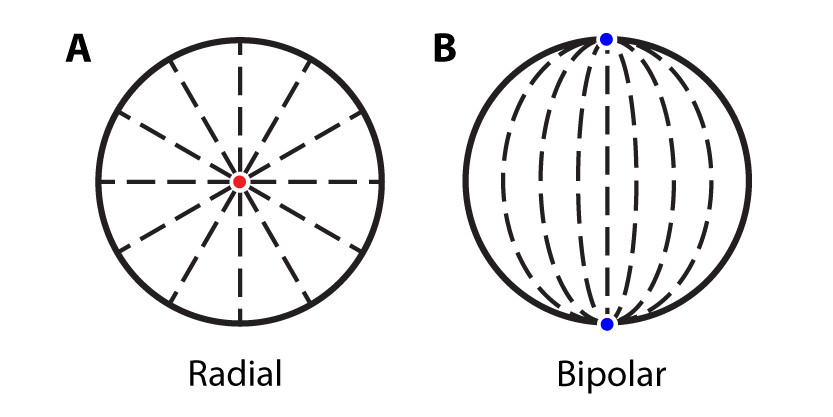
\includegraphics{figures/C2/Ch2-Figs_DropSchem.png}
  \caption{Nematic liquid crystal confined to a spherical volume.
  (A), The classic radial director configuration found under homeotropic boundary conditions.
  The defect is indicated by ${\color{red} \bullet}$.
  (B), The classic bipolar director configuration found under degenerate planar boundary conditions.
  The 2 defects are indicated by ${\color{blue} \bullet}$.}\label{f:2-DropSchem}
\end{figure}

\begin{figure}[h]
  \centering
  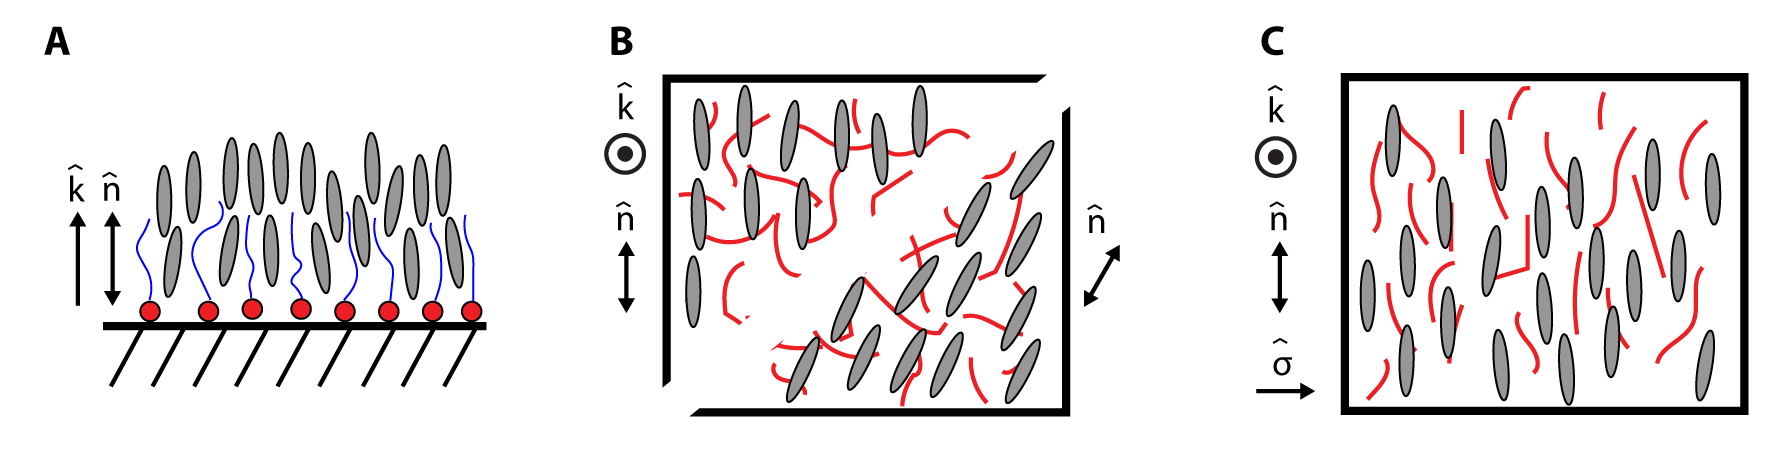
\includegraphics{figures/C2/Ch2-Figs_Anchor.png}
  \caption{Common anchoring schemes for nematic liquid crystals. (A), Homeotropic anchoring enforced by surfactant molecules.
  The polar heads of the molecules adsorb to the substrate, with the nonpolar tails extending into the NLC.
  The tails serve to align the nematic mesogens along the surface normal, making $\mathbf{k} \parallel \mathbf{n}$, as seen in the schematic.
  (B), Degenerate planar anchoring enforced by randomly oriented polymers on the substrate. The polymers only require that the mesogens lie in the plane of the interface such that $\mathbf{k} \perp \mathbf{n}$. Since there is no preferred direction in the plane of the substrate, the mesogens are free to choose any director in the plane, as depicted in the schematic.
  (C), Planar anchoring enforced via aligned polymers on the substrate. Here, the polymers have an alignment direction, setting the direction that the NLC mesogens also prefer to align along, such that $\mathbf{n} \parallel \bm{\sigma}$, where $\bm{\sigma}$ is a vector describing the polymer alignment direction, as defined in the schematic.}\label{f:2-Anchor}
\end{figure}

In an experiment, confinement takes place with either solid boundaries, such as glass cells and capillaries, or fluid boundaries such as in emulsions of a nematic material dispersed in an outer immiscible liquid phase.
It is also possible to confine a nematic using both solid boundaries and fluid boundaries, as with a droplet of NLC sitting on a solid base.
In such a sessile drop, the solid boundary provides a flat base for the NLC;\@ however, the remainder of the confinement is provided by the free surface, where the NLC is in contact with air.
In general, a NLC in contact with an arbitrary boundary will be subject to degenerate tilt boundary conditions.
Thus, for experiments that require a specific boundary condition we must treat the interface.\\

In order to discuss specific strategies for enforcing anchoring, we must first narrow down the compounds that might be used.
NLC can be divided into two broad categories, thermotropics and lyotropics~\cite{RN33}.
In thermotropic LC's, temperature is an important control parameter.
If the temperature is too high, the nematic phase will melt to the isotropic phase and if the temperature is too low, the nematic phase will phase transition to a less symmetric LC phase or to a crystalline phase.
Lyotropic LC's are suspensions of particles in a solvent and therefore are sensitive to both concentration as well as to temperature.

In this Thesis, we will primarily use 4-cyano-4'-pentylbiphenyl (5CB), a thermotropic liquid crystal whose mesogens are $\sim 2$ nm long~\cite{RN33}.\@
5CB belongs to the cyanobiphenyl family of NLC, which are characterized by a cyano (CN) group  bonded to a biphenyl (C$_6$H$_4$)(C$_6$H$_4$) group bonded to an alkyl group of given length, C$_p$H$_{2p+1}$, where $p$ is the number of carbon atoms in the group~\cite{RN33}.
In the case of 5CB, the chemical formula is: (CN)(C$_6$H$_4$)(C$_6$H$_4$)(C$_5$H$_{11}$).
Thus, we see that the ``5'' in 5CB refers to the number of carbon atoms in the alkyl group.
Since the different cyanobiphenyls generally only differ in the number of carbon atoms in the alkyl group, the anchoring techniques we cover below for 5CB are general and should apply to any $p$CB.

To enforce homeotropic anchoring for 5CB against a smooth, isotropic solid boundary such as a glass capillary or glass slide, it is common to either deposit surfactant molecules or bond silanes to the surface.
In both cases, the smooth surface becomes decorated with long chains that stick up normal to the surface.
The nematic mesogens at the surface are aligned by the chains, enforcing homeotropic anchoring at the surface~\cite{RN33}, as seen schematically in Figure~\ref{f:2-Anchor}(A).
For example, to enforce homeotropic anchoring for 5CB on glass, we dip coat glass slides in a $0.1$\% w/w lecithin in hexane solution and then let the slides dry.
When the hexane evaporates, the polar head of the lecithin molecule is attached to the glass surface, leaving the long tails sticking up from the glass~\cite{RN140}.

Similarly, it is common to enforce homeotropic anchoring in solution again using surfactants.
Here, for an organic NLC dispersed in an aqueous phase, the polar head of the surfactant sits in the aqueous phase while the hydrophobic tail inserts itself into the NLC volume, aligning the NLC at the interface~\cite{RN150,RN235}.
For example, we use sodium dodecyl sulfate (SDS) in water to enforce homeotropic anchoring in 5CB emulsions and liquid bridges.
While homeotropic anchoring can be enforced with as little as 1 mM SDS in H$_2$O, we use a solution of 8 mM SDS in H$_2$O for the strongest possible anchoring~\cite{RN235}.
At concentrations above 8 mM, SDS forms micelles in H$_2$O such that working with higher concentrations does not yield any more free SDS in the solution that could potentially adsorb to the interface and contribute to a larger anchoring strength~\cite{RN234}.
This concentration is known as the critical micelle concentration (CMC) and is a common feature in solutions of surfactants or other amphiphilic molecules~\cite{RN233,RN234}. \\

While smooth, isotropic solid boundaries can exhibit degenerate planar anchoring, in general the anchoring will be degenerate and tilted.
Thus, surface is often coated with a polymer such that the polymer orientations on the surface are random.
Since the polymers have no preferred alignment in the plane of the surface, the mesogens are free to choose their own director in the plane~\cite{RN313}, as seen schematically in Figure~\ref{f:2-Anchor}(B).

% For example, electrospinning poly(vinyl alcohol) (PVA) or poly(ethylene oxide) (PEO) onto glass yields degenerate planar anchoring for 5CB~\fxnote{reference}.
If a preferred anchoring direction in the plane, $\bm{\sigma}$, is desired, the polymer coating can be rubbed along $\bm{\sigma}$, aligning the polymers and creating ``grooves'' in the polymer coating along the rubbing direction, as seen schematically in Figure~\ref{f:2-Anchor}(C).
The NLC will the align along the rubbing direction, breaking the degeneracy in the anchoring~\cite{RN33,}.
Note that rubbed polymer surfaces do not have perfect planar anchoring but rather exhibit a small tilt angle~\cite{RN232}.
Thus, when designing planar-aligned liquid crystalline cells, where the NLC is confined between two parallel plates with planar anchoring, the rubbing direction on the plates will be anti-parallel.
The anti-parallel rubbing aligns the tilt angles at the plates such that the NLC can still form a homogeneously-aligned domain between the plates~\cite{RN232}. \\

For dispersions of organic NLC droplets such as 5CB in a continuous aqueous phase, we add a polymer like PEO or PVA to the aqueous phase~\cite{RN105,RN93}.
The polymer adsorbs to the interface between the NLC and the continuous phase, giving degenerate planar anchoring.
We know of no easy way to break the planar degeneracy in the anchoring when dealing with a liquid-liquid interface.
In addition, we note that even though 5CB exhibits degenerate planar anchoring at the interface with pure water, the addition of a polymer strengthens the anchoring as well as acting to stabilize the emulsion when 5CB droplets are dispersed in H$_2$O~\cite{RN105,RN93}.\\




\subsection{Birefringence and optically polarized microscopy}
Once the nematic is confined in the desired volume with the desired boundary conditions, the most common way to study the sample is with optical polarized microscopy.
This technique takes advantage of the birefringence of the NLC to determine the director in the sample.
For a uniaxial nematic, the index of refraction along $\mathbf{n}$ is known as the ``extraordinary index of refraction'', denoted $n_E$, and the index of refraction perpendicular to $\mathbf{n}$ is called the ``ordinary index of refraction'', denoted as $n_o$.
Since the index of refraction along $\mathbf{n}$ is $n_E$, the director also serves as the optic axis of uniaxial nematics~\cite{RN232}.
The birefringence is defined as $\Delta n = n_E-n_o$~\cite{RN232}.
If $n_E > n_o$, $\Delta n > 0$ and the material has positive birefringence.
Conversely, if $\Delta n < 0$, the material has negative birefringence.
Thus, the index of refraction affecting the incident light on a birefringent material will depend on the polarization of the light relative to $\mathbf{n}$~\cite{RN232}.

While unpolarized light will be unaffected by the birefringent material, in general polarized light will have its polarization state affected.
Consider linearly polarized light incident upon a birefringent material with $n_E$ along $\hat{x}$ and $n_o$ along $\hat{y}$.
If the incident light is polarized along $\hat{x}$ or $\hat{y}$, it will encounter only either the extraordinary index of refraction or the ordinary index of refraction and will leave the birefringent volume with no change in its polarization state.
However, now let the incident light be linearly polarized at $45^o$.
In this case, the incident light can be decomposed into one component along $\hat{x}$ and another component along $\hat{y}$.
Since each component will see a different index of refraction, they will propagate at different speeds, creating a phase difference between the two components of the incident light.

This phase difference is known as the retardation and is given in multiples of $2 \pi$ by $\Gamma = 2 \pi \Delta n \, d / \lambda$, where $d$ is the thickness of the birefringent material, and $\lambda$ is the wavelength of the incident light in vacuum~\cite{RN232}.
For our example of incident light linearly polarized at $45^o$, let $\Delta n \, d = \lambda / 2$ such that $\Gamma =  \pi$.
The light after leaving the sample will now be polarized at $-45^o$, and the birefringent material has the properties of a half-waveplate~\cite{RN232}.
Similarly, if $\Delta n \, d = \lambda$, $\Gamma =  2 \pi$, the birefringent material is a full-waveplate and the output light will be unchanged~\cite{RN232}.\\

\begin{figure}[h]
  \centering
  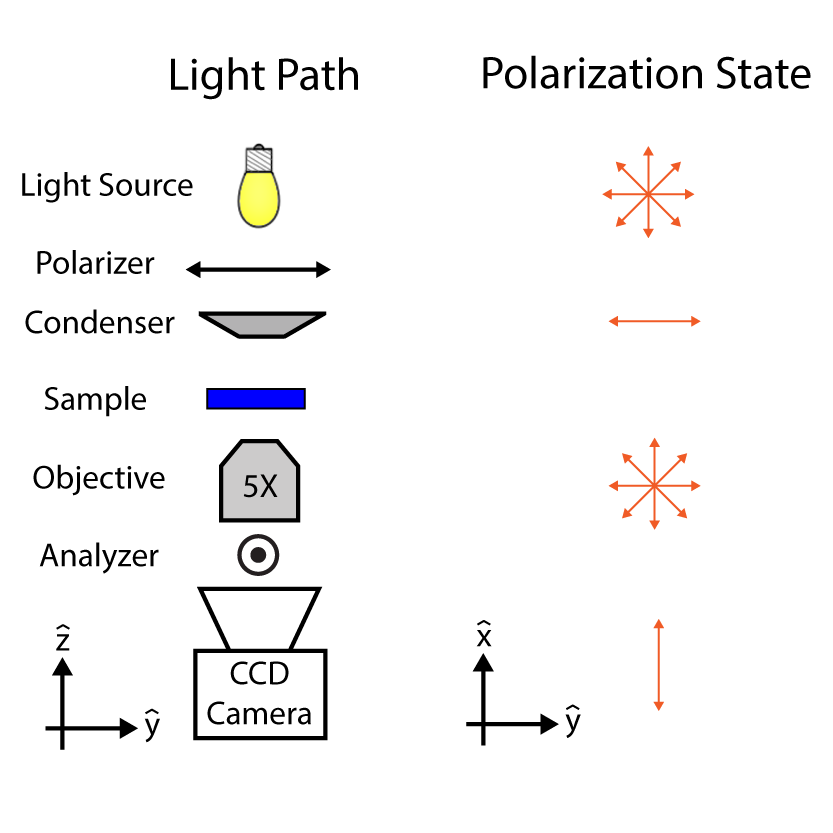
\includegraphics{figures/C2/Ch2-Figs_OPMSchem.png}
  \caption{Schematic of the light path and polarization state for optically polarized microscopy (OPM). OPM places a linear polarizer called the ``polarizer'' before the condenser and another linear polarizer called the ``analyzer'' after the objective. The polarization states depicted in the figure assume the sample is birefringent and the pass axes of the polarizer and the analyzer are orthogonal.}\label{f:2-OPMSchem}
\end{figure}

\begin{figure}[h]
  \centering
  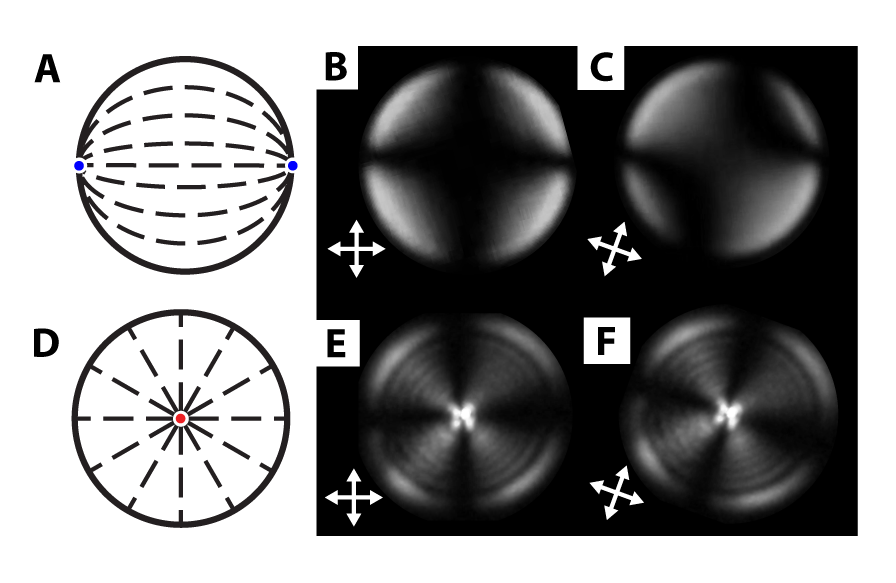
\includegraphics{figures/C2/Ch2-Figs_OPMDrops.png}
  \caption{Example OPM textures for a bipolar drop and a radial drop.
  (A--C), schematic and textures for a radial drop.
  The textures in (B,C) have the polarizer and analyzer directions specified on the images, with the drops oriented as depicted in (A).
  Note how the texture only changes orientation with the polarizer and analyzer orientation, but does not change character.
  (D--F), schematic and texture for a bipolar drop.
  The textures in (E,F) have the polarizer and analyzer directions specified on the images, with the drops oriented as depicted in (D).
  Note how the texture changes as the polarizer and analyzer rotate.
  }\label{f:2-OPMDrops}
\end{figure}

Optical polarized microscopy (OPM) takes advantage of birefringence and turns the change in polarization into changes in transmitted intensity.
The typical setup uses a pair of linear polarizers into the light path of a standard wide-field optical microscope.
A linear polarizer is an optical element that only passes light polarized along a specific axis known as the ``pass axis''~\cite{RN232}.
Thus, unpolarized light incident upon a linear polarizer will have its intensity reduced by half and the output light will be linearly polarized along the pass axis of the polarizer.
Illustrating the light path for optical polarized microscopy, the incident light passes through the first linear polarizer, known as the ``polarizer'', through the sample, through the objective, and through the second linear polarizer, known as the ``analyzer'', before it is incident on the eyepiece or the camera used to capture the microscope image~\cite{RN232}.
The light path is illustrated schematically in Figure~\ref{f:2-OPMSchem}.
If the polarizer and analyzer are ``crossed,'' or oriented with their pass axes orthogonal to each other, any isotropic sample will be entirely dark.
This is because the sample does not affect the polarization state of the incident light such that the linearly polarized light from the polarizer is blocked by the analyzer.
However, if the sample is birefringent, the polarization state of the incident light will change and some of the light will pass through the analyzer and be transmitted onto the eyepiece or camera.
This is illustrated in the schematic in Figure~\ref{f:2-OPMSchem}.

The intensity pattern in the image output from an OPM setup can then be used to deduce information about the sample.
While for our purposes we typically care about the spatial variation of the optic axis, and thus the spatial variation in $\mathbf{n}$, OPM can also be used to determine the birefringence of the sample~\cite{RN232}.
For example, we consider 5CB confined to spherical nematic droplets.
Under homeotropic anchoring the droplet will have the classic ``radial'' director field [see Figure~\ref{f:2-OPMDrops}(A)] while under degenerate planar anchoring the droplet will have the classic ``bipolar'' configuration [see Figure~\ref{f:2-OPMDrops}(D)]~\cite{RN177}.
These configurations can be distinguished by their OPM textures, as seen in Figure~\ref{f:2-OPMDrops}(B,C) for a radial drop and Figure~\ref{f:2-OPMDrops}(E,F) for a bipolar drop.
Note how the light and dark portions of the bipolar texture change from Figure~\ref{f:2-OPMDrops}(E) to Figure~\ref{f:2-OPMDrops}(F) as the polarizer and analyzer change orientation, while still crossed.
The radial texture only rotates with the polarizer and analyzer but does not change in the frame of the polarizer and analyzer; see Figure~\ref{f:2-OPMDrops}(B,C).

\begin{table}[t]
  \centering
\caption{Basic group theory definitions~\cite{RN320,RN319}.}
\begin{tabular}{|r l|}
\hline
{\bf set}:& A collection of objects\\[10 pt]
{\bf group}:& \begin{minipage}[t]{0.65\textwidth}
A set, $\Sigma$, and a binary operation, or group multiplication, $\cdot$, that combines two elements in the set to form a third element in the set, satisfying:
    \begin{itemize}
      \item[]{\bf associativity}: $\forall \; a,b,c \in \Sigma$, $(a \cdot b) \cdot c = a \cdot (b \cdot c)$.
      \item[]{\bf identity}: $\exists! \; e \in \Sigma$ s.t. $\forall \; a \in G, \, a\cdot e=e \cdot a = a$.
      \item[]{\bf invertability}: $\forall \; a \in \Sigma$, $\exists! \; a^{-1} \in \Sigma$ s.t. $a a^{-1} = a^{-1} a = e$, with $e$ the identity.
    \end{itemize}
    If $\forall \; a,b \in \Sigma, \, a \cdot b = b \cdot a$, the group is said to be Abelian.
    Note that the requirement $\forall \; a,b \in \Sigma, \; a \cdot b \in \Sigma$ is known as {\bf closure}.\\
\end{minipage}\\
{\bf Lie group}:& \begin{minipage}[t]{0.65\textwidth}
A group that is also a differentiable manifold, whose group operation is also differentiable. Lie groups are associated with continuous symmetries, for example, SO(3), the set of all rotations in 3D Euclidean space under multiplication. Other common Lie groups include $n$-dimensional Euclidean space $\mathbb{R}^n$ under vector addition, and GL(2), the group of $2 \times 2$ invertible matrices, also under multiplication.\\
\end{minipage}\\
{\bf discrete group}:& \begin{minipage}[t]{0.65\textwidth}
A group whose elements must be countable. This is instantly satisfied if there are a finite number of elements in the group. In this case the order of the group is given by the number of elements in the group. If there are an infinite number of elements, there must be a one-to-one mapping from the elements to the integers.\\
\end{minipage}\\
{\bf homomorphism}:& \begin{minipage}[t]{0.65\textwidth}
A structure-preserving map, $\varphi$, between the groups $G$ and $H$, $\varphi : G \to H$. A homomorphism must satisfy, $\forall \; a, b \in G$, $\varphi(a \cdot b) = \varphi(a) \cdot \varphi(b)$. Since $\forall \; a \in G, \; \varphi(a) \in H$, we see that a homomorphism preserves the group multiplication. A homomorphism is not necessarily a one-to-one mapping. If the homomorphism is one-to-one, then the homeomorphism is an {\bf isomorphism}.\\
\end{minipage}\\
\hline
\end{tabular}
\label{t:2-GroupTheory}
\end{table}
